\documentclass[a4paper,12pt]{article}
\usepackage[OT1]{fontenc}
\usepackage{times}
\usepackage[english]{babel}
\usepackage[most]{tcolorbox} % 'most' includes all libraries
\usepackage{xcolor}
\usepackage{enumitem}
\usepackage{float}
\usepackage{geometry}
\geometry{top=20mm}
\geometry{bottom=20mm}
\geometry{left=10mm}
\geometry{right=20mm}
\usepackage{charter}

% Define custom boxes
\newtcolorbox{infobox}{
  colback=blue!5!white,
  colframe=blue!75!black,
  title=Information,
  fonttitle=\bfseries,
  boxrule=0pt,
  arc=0mm
}

\newtcolorbox{warningbox}{
  colback=yellow!5!white,
  colframe=yellow!75!black,
  title=Warning,
  fonttitle=\bfseries,
  boxrule=0pt,
  arc=0mm
}

\newtcolorbox{importantbox}{
  colback=red!5!white,
  colframe=red!75!black,
  title=Important,
  fonttitle=\bfseries,
  boxrule=0pt,
  arc=0mm
}

%\begin{infobox}
%  This is an information box with useful tips.
%\end{infobox}
%
%\begin{warningbox}
%  This is a warning box. Be careful!
%\end{warningbox}
%
%\begin{importantbox}
%  This is an important notice.
%\end{importantbox}

\setlength{\itemsep}{0pt} % Set the space between items to zero
%\DeclareGraphicsExtensions{.png}
%\usepackage{algorithmic}
\graphicspath{}
%opening
\begin{document}
  \begin{center}
    \vspace*{0.4\textheight}
    \Huge{Edit\_geo} \normalsize
    \vfill
    Author: Shtyrkhunov Nikita\\
    email: nv.shtyrkhunov@gmail.com\\
    \vspace{0.05\textheight}
    16.12.2025
  \end{center}

  \newpage
  \section{Introduction}

  \subsection{Overview}
  This script is designed to modify a computational mesh stored in a {\tt .geo} file, generated by {\tt Carre2}. The script is located in the {\tt \$\{SOLPSTOP\}/scripts/Matlab\_SPb} folder.

  This script provides the following functionalities:
  \begin{enumerate}[itemsep=2pt,topsep=5pt]
    \item Examine face and cell types
    \item Move vertices strictly along a poloidal direction or in any arbitrary direction
    \item Move an entire poloidal line
    \item Assign a face label ({\tt fcLbl}) to any desired face
    \item Reposition a grid line from one vertex to another
    \item Add or remove cells by merging or splitting vertices
  \end{enumerate}

  When executing the script, you will be prompted to select a file through the file explorer. This file must have the {\tt .geo} extension. You will then see a display similar to Figure~\ref{fig:init}.
  \begin{figure}[H]
    \centering
    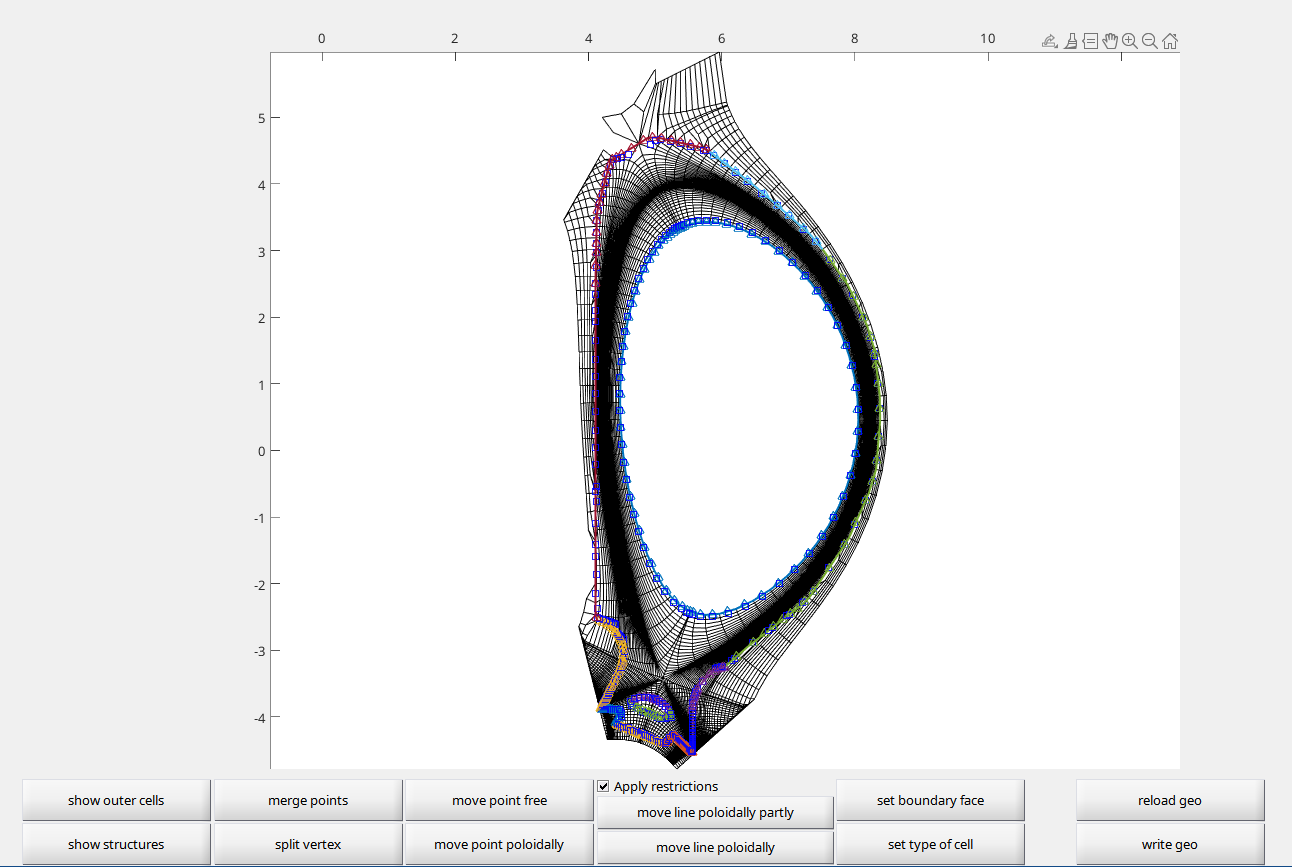
\includegraphics[width=0.7\linewidth]{pictures/init}
    \caption{Initial mesh visualization}
    \label{fig:init}
  \end{figure}

  \subsection{Designations}

  \begin{itemize}[itemsep=2pt,topsep=5pt]
    \item {\bf Blue squares} Boundary cells
    \item {\bf Blue circles} Outer cells (invisible by default)
    \item {\bf Triangles of different colour} Boundary faces (with their {\tt fcLbl} boundary number displayed if you select them)
    \item {\bf Coloured cell faces} Boundary faces
    \item {\bf Coloured bold lines} Structures which were used to construct the mesh
  \end{itemize}

  \begin{infobox}
    To show structures, a {\tt structure.dat} or {\tt vessel.dat} file must be present in the same directory as your {\tt .geo} mesh file.
  \end{infobox}

  \section{Program Options}

  \subsection{Show outer cells}

  This option toggles the visibility of markers for outer cells. \\

  \textbf{Procedure:}
  \begin{enumerate}[itemsep=2pt,topsep=5pt]
    \item Click the button to show markers if they are hidden
    \item Click the button to hide markers if they are shown
  \end{enumerate}

  \subsection{Show structures}

  This option toggles the visibility of physical structures (e.g., vessel walls) used in mesh generation. \\

  \textbf{Procedure:}
  \begin{enumerate}[itemsep=2pt,topsep=5pt]
    \item Click the button to show structures if they are hidden
    \item Click the button to hide structures if they are shown
  \end{enumerate}

  \subsection{Merge points}

  This option merges two vertices into one. \\

  \textbf{Procedure:}
  \begin{enumerate}[itemsep=2pt,topsep=5pt]
    \item Click the corresponding button. A selection cursor will appear.
    \item Select the first vertex to merge (left-click).
    \item Select the target vertex where they should merge (left-click).
  \end{enumerate}
  The two vertices will merge into a single vertex located at the coordinates of the second selected vertex.

  \subsection{Split vertex}

  This option extracts the vertex of one cell from a vertex shared by multiple cells, creating a new separate vertex. \\

  \textbf{Procedure:}
  \begin{enumerate}[itemsep=2pt,topsep=5pt]
    \item Click the corresponding button. A selection cursor will appear.
    \item Place the cursor {\em inside the cell} you wish to modify, near the shared vertex to be split, and left-click.
    \item Move the new cursor to the desired location for the extracted vertex and left-click.
  \end{enumerate}

  \subsection{Move point poloidally}

  This option moves a vertex along a poloidal direction (following a flux surface). \\

  \textbf{Procedure:}
  \begin{enumerate}[itemsep=2pt,topsep=5pt]
    \item Click the corresponding button. A selection cursor will appear.
    \item Move the cursor near the vertex you wish to move and left-click.
    \item Move the new cursor to the target vertex location along the flux surface and left-click.
  \end{enumerate}

  The vertex will move along its flux surface to the point closest to your selected target.

  \subsection{Move point free}

  This option moves a vertex to any arbitrary location. The procedure is identical to {\tt Move Point poloidally}, but the vertex moves precisely to the selected coordinates.

  \begin{warningbox}
    This operation can distort flux surfaces. It is recommended to use it only for boundary vertices.
  \end{warningbox}

  \subsection{Move line poloidally}

  This option moves all vertices on a selected radial line along their respective flux surfaces. \\

  \textbf{Procedure:}
  \begin{enumerate}[itemsep=2pt,topsep=5pt]
    \item Click the corresponding button. A selection cursor will appear.
    \item Move the cursor near a vertex on the desired radial line and left-click.
    \item Move the new cursor to the target location and left-click.
  \end{enumerate}
  All vertices on that radial line will move along their flux surfaces by the same poloidal displacement, defined by the movement of the first selected vertex.

  \subsection{Move line poloidally partly}

  This option is similar to {\tt Move Line Poloidally} but allows you to specify a subset of vertices to move. \\

  \textbf{Procedure:}
  \begin{enumerate}[itemsep=2pt,topsep=5pt]
    \item Click the corresponding button. A selection cursor will appear.
    \item Select the first vertex to move (left-click).
    \item Select the target location for this vertex (left-click). This defines the displacement vector.
    \item Select the last vertex in the range to be moved (left-click).
  \end{enumerate}
  All vertices from the first to the last selected will move along their flux surfaces by the same distance.

  \begin{infobox}
    The {\tt Apply restrictions} option applies to both {\tt Move Line Poloidally} operations. It prevents vertices from moving outside their cell boundaries. However, if neighbouring cells in a flux tube differ significantly in size, this restriction may be too severe. In such cases, you can disable restrictions and proceed with caution.
  \end{infobox}

  \subsection{Set boundary face}

  This option allows to change the label number of boundary faces for one or several faces at a time. \\

  \textbf{Procedure:}
  \begin{enumerate}[itemsep=2pt,topsep=5pt]
    \item Click the corresponding button. A selection cursor will appear.
    \item Move the cursor to a face whose label you wish to change (within the adjacent boundary cell) and left-click.
    \item Repeat for all faces to be modified. To finalize the selection, press the {\em middle mouse button} on the last face.
    \item An input dialog will appear. Enter the desired label number (an integer; use {\tt 0} to remove a boundary face label) and click {\tt OK}.
  \end{enumerate}

  \begin{importantbox}
    A face always belongs to both cells it bounds. You should click in the boundary cell (they are marked with blue squares) near the face. \\
    Recall also that faces with the same label number should form a continuous polygon.
  \end{importantbox}

  \subsection{Set type of cell}

  This option allows you to change the type of specified cells. \\

  Available cell types are:
  \begin{itemize}[itemsep=2pt,topsep=5pt]
    \item {\bf Inner} The cell is inside the computational domain and has no contact with its edge.
    \item {\bf Boundary} The cell lies at the edge of the computational domain (but still inside it).
    \item {\bf Outer} The cell lies outside the computational domain and will not be used to construct the {\tt B2.5} mesh.
  \end{itemize}

  \textbf{Procedure:}
  \begin{enumerate}[itemsep=2pt,topsep=5pt]
    \item Click the corresponding button. A selection cursor will appear.
    \item Move the cursor inside a cell whose type you wish to change and left-click.
    \item Repeat for all cells to be modified. To finalize the selection, press the {\em middle mouse button} on the last cell.
    \item A list dialog will appear. Select the desired cell type. If you select {\tt Boundary}, you will be prompted to enter a boundary label number for that cell.
  \end{enumerate}

  \begin{importantbox}
    If you select the {\tt Boundary} type, ensure you follow the face-selection rules outlined in the {\tt Set Boundary Face} option.
  \end{importantbox}

  \subsection{Reload geo}

  This option reloads the mesh from the most recently saved {\tt .geo} file, discarding any unsaved modifications.

  \subsection{Write geo}

  This option saves the current mesh to a {\tt .geo} file. You can choose to save it as a new file or overwrite the previously saved one.

  \begin{infobox}
    It is recommended to save the mesh to a {\em new {\tt .geo} file} before performing any modifications that are difficult to revert (e.g., moving points/lines, merging/splitting vertices).
  \end{infobox}

  \section{Example of Usage}

  This section demonstrates mesh editing for an ITER configuration. \\

  First, open the mesh (see Figure~\ref{fig:init}). Typically, I inspect the mesh for the following issues:
  \begin{itemize}
    \item Areas with large variations in neighboring cell sizes
    \item Flux tubes where boundary cells are too narrow relative to the flux tube width
    \item Very short flux tubes (2-3 cells per flux tube)
    \item Errors in boundary definition (e.g., boundary faces appearing between two inner cells)
  \end{itemize}

  \subsection{First Issue: Small Cells in the X-Point Region}

  Initially, I identified small cells in the X-point region (see Figure~\ref{fig:moveline1}).
  \begin{figure}[H]
    \centering
    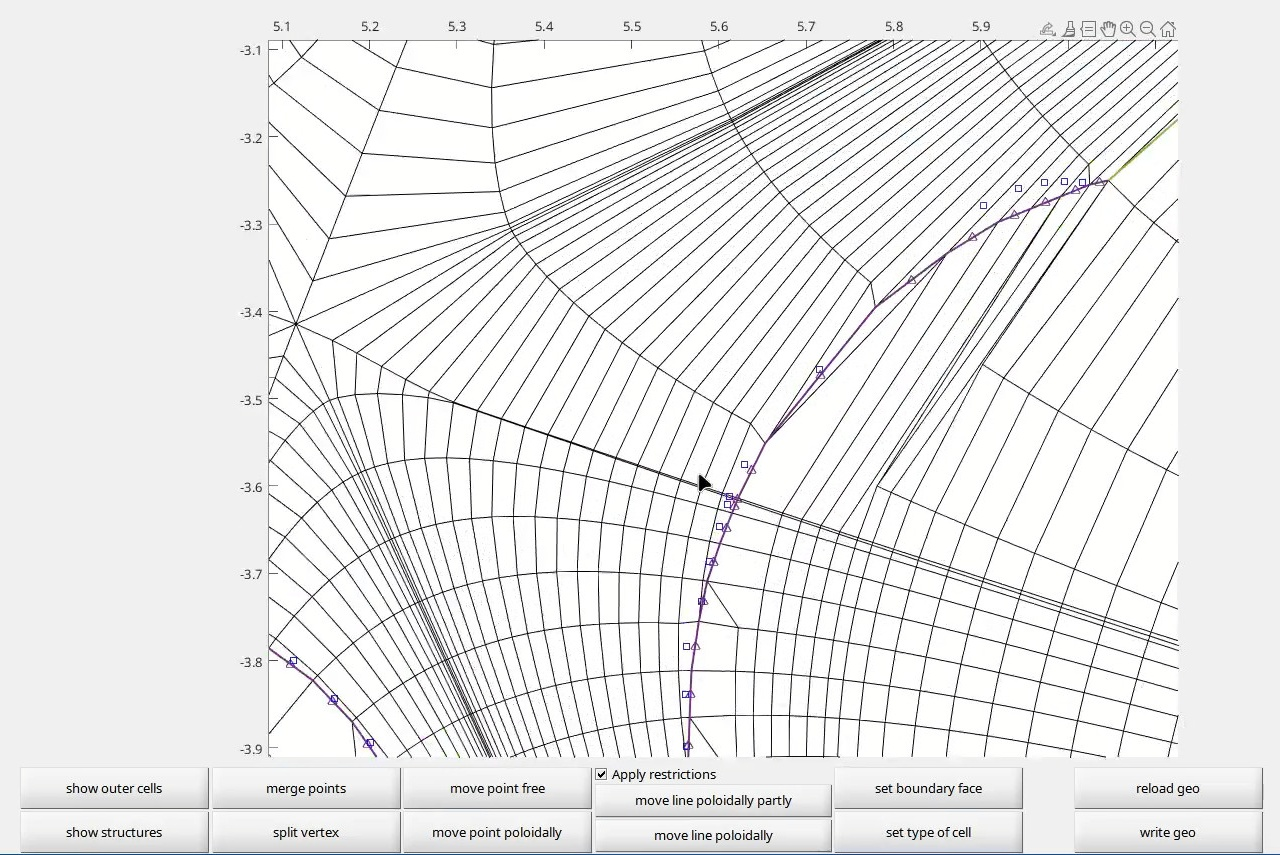
\includegraphics[width=0.33\linewidth]{pictures/move_line1}
    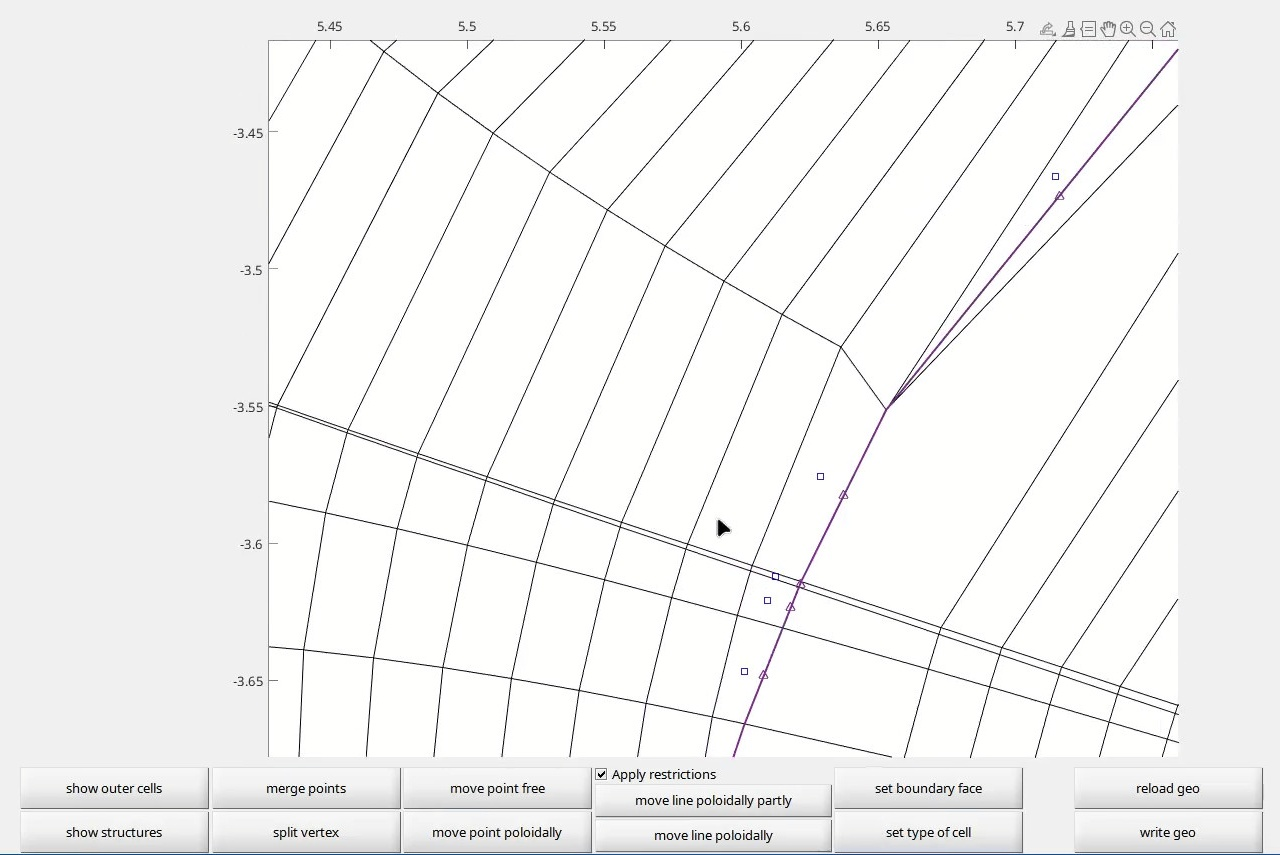
\includegraphics[width=0.33\linewidth]{pictures/move_line2}
    \caption{Small cells in X-point region (indicated by arrows)}
    \label{fig:moveline1}
  \end{figure}

  I used the {\tt Move Line Poloidally Partly} option to enlarge these cells. Figure~\ref{fig:moveline_example} illustrates the procedure, showing the selected points and resulting line movement.

  \begin{figure}[H]
    \centering
    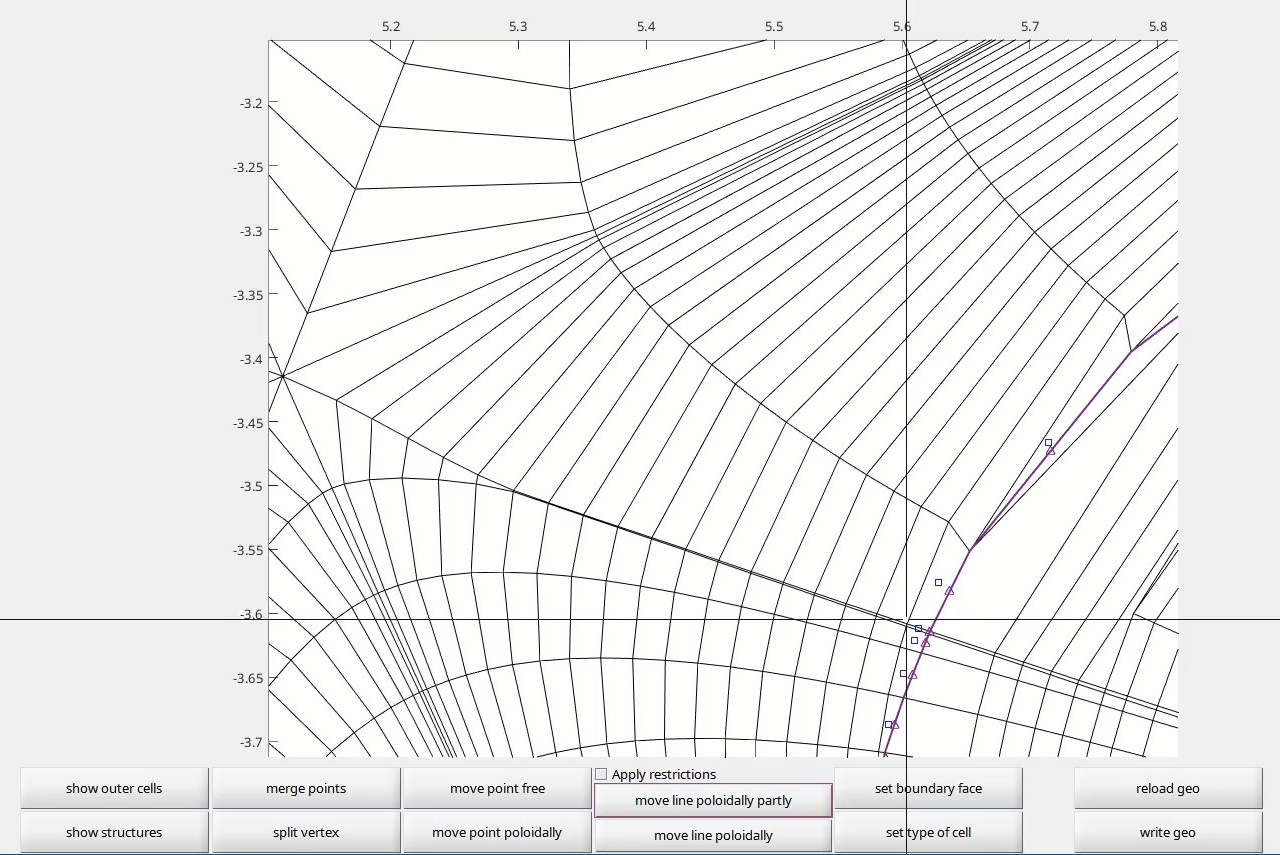
\includegraphics[width=0.245\linewidth]{pictures/move_line3}
    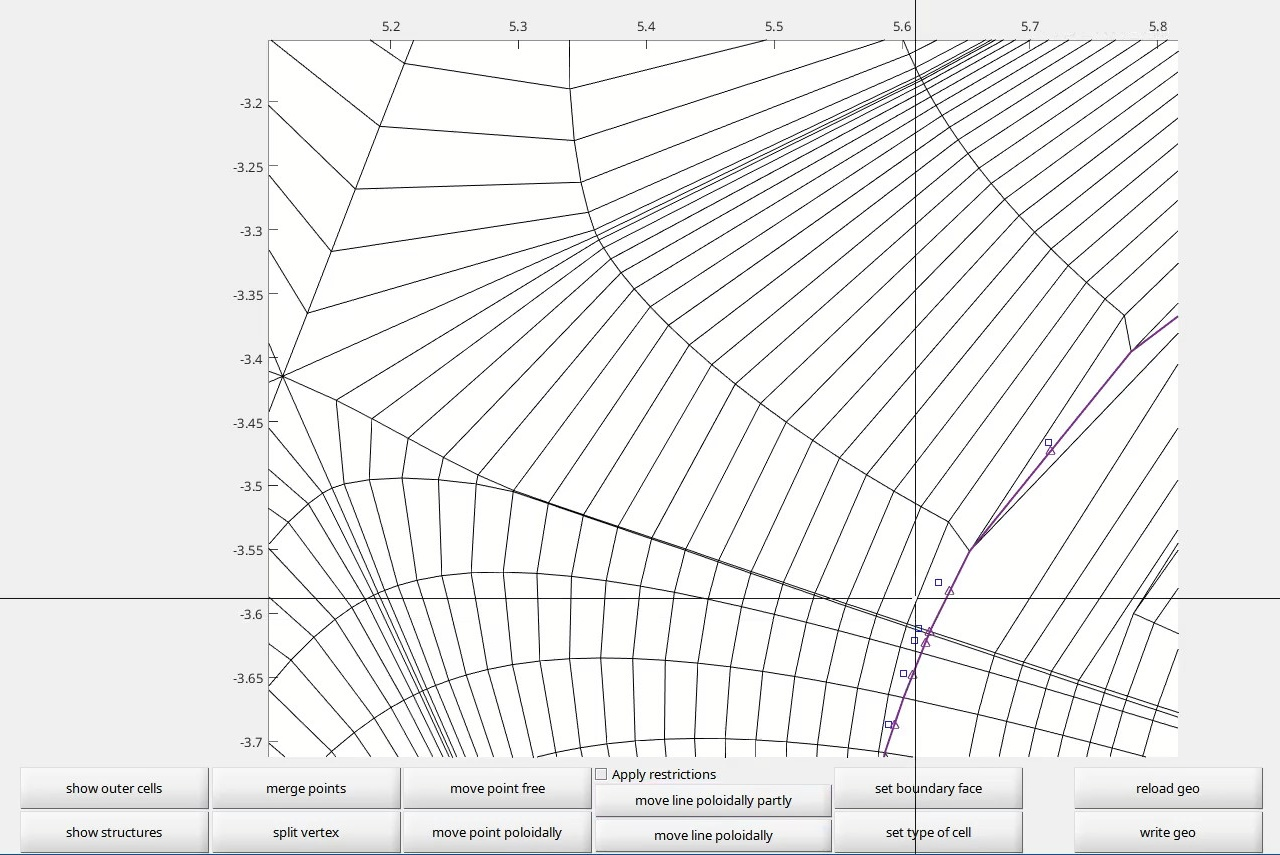
\includegraphics[width=0.245\linewidth]{pictures/move_line4}
    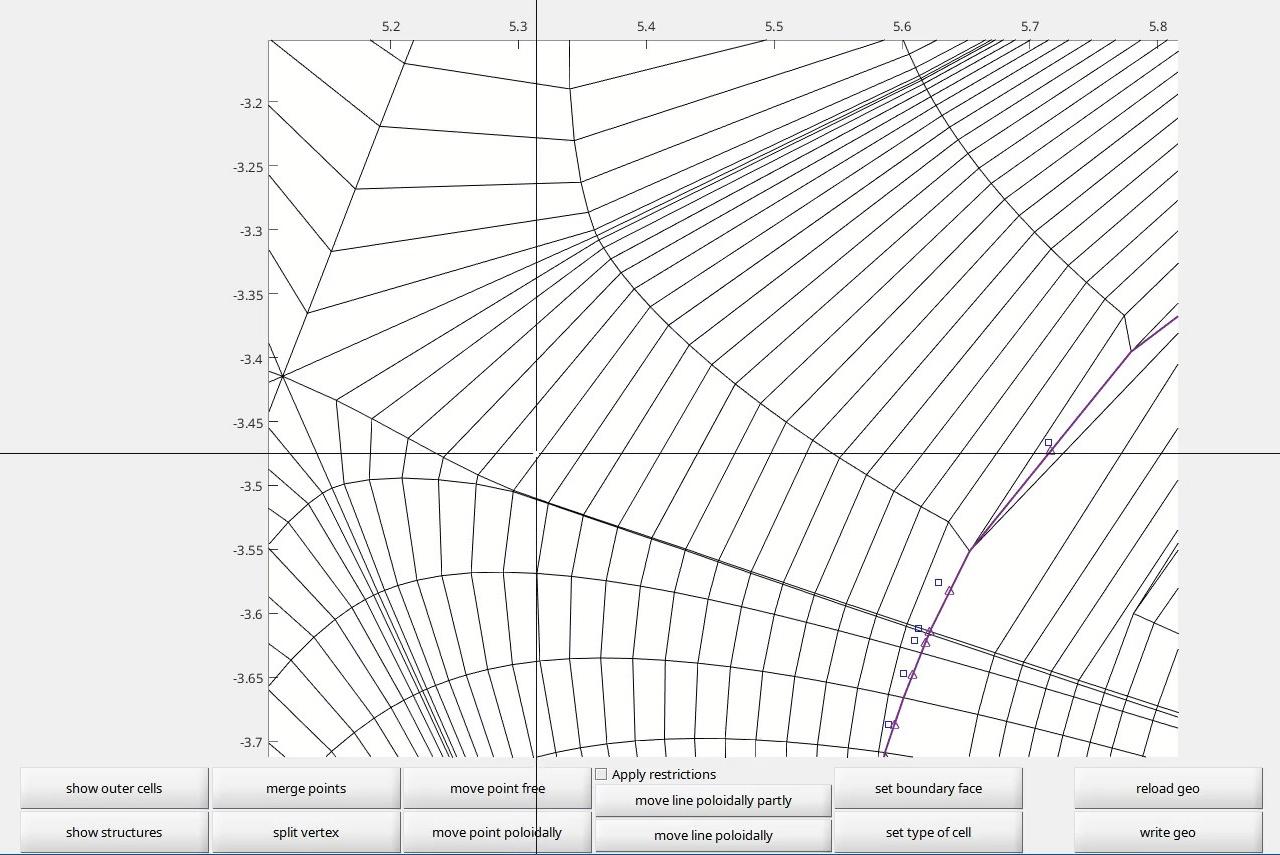
\includegraphics[width=0.245\linewidth]{pictures/move_line5}
    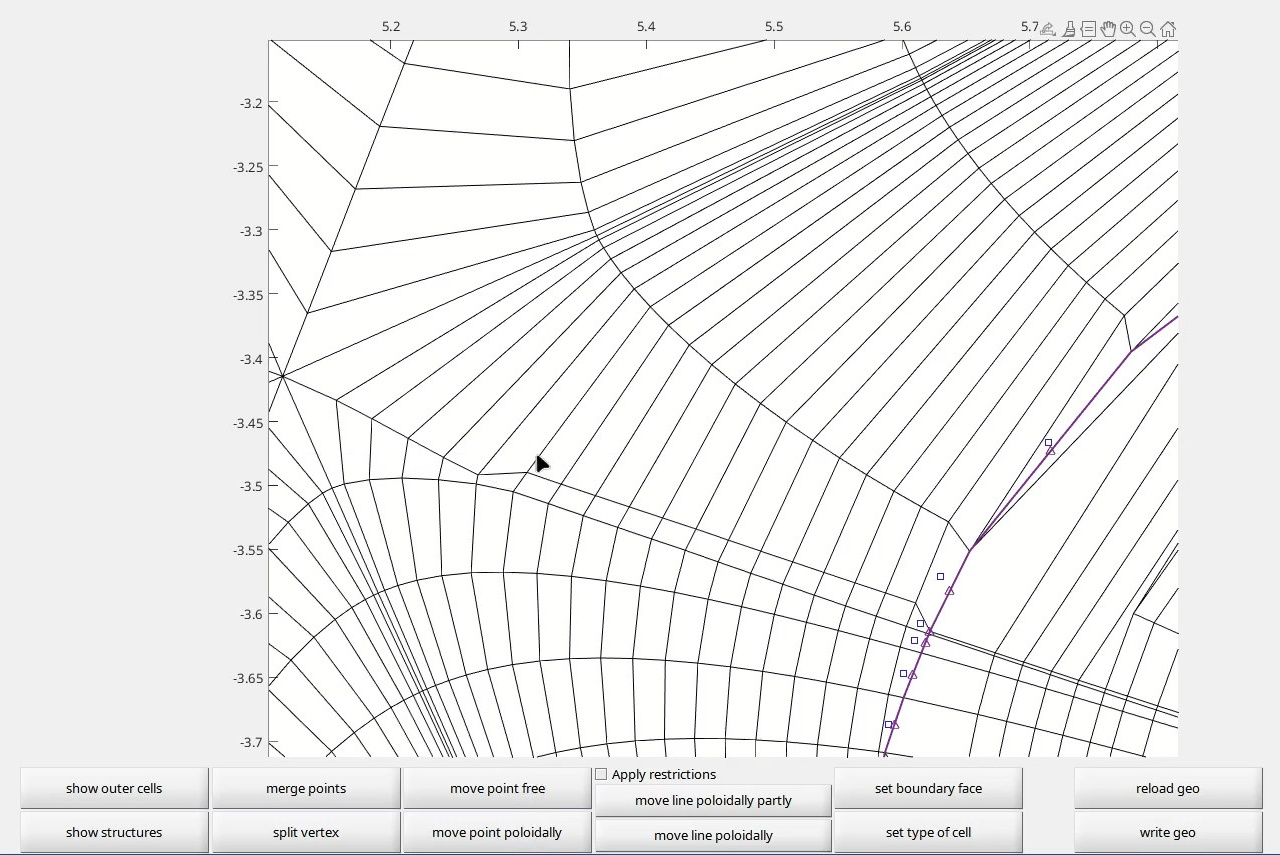
\includegraphics[width=0.245\linewidth]{pictures/move_line6}
    \caption{Sequence for moving a line poloidally: (a) Select first vertex, (b) Select target location, (c) Select last vertex, (d) Result}
    \label{fig:moveline_example}
  \end{figure}

  Note that {\tt Move Line Poloidally} does not move boundary faces automatically. These must be adjusted separately using {\tt Move Point Poloidally}, as shown in Figure~\ref{fig:movepoint_example}.

  \begin{figure}[H]
    \centering
    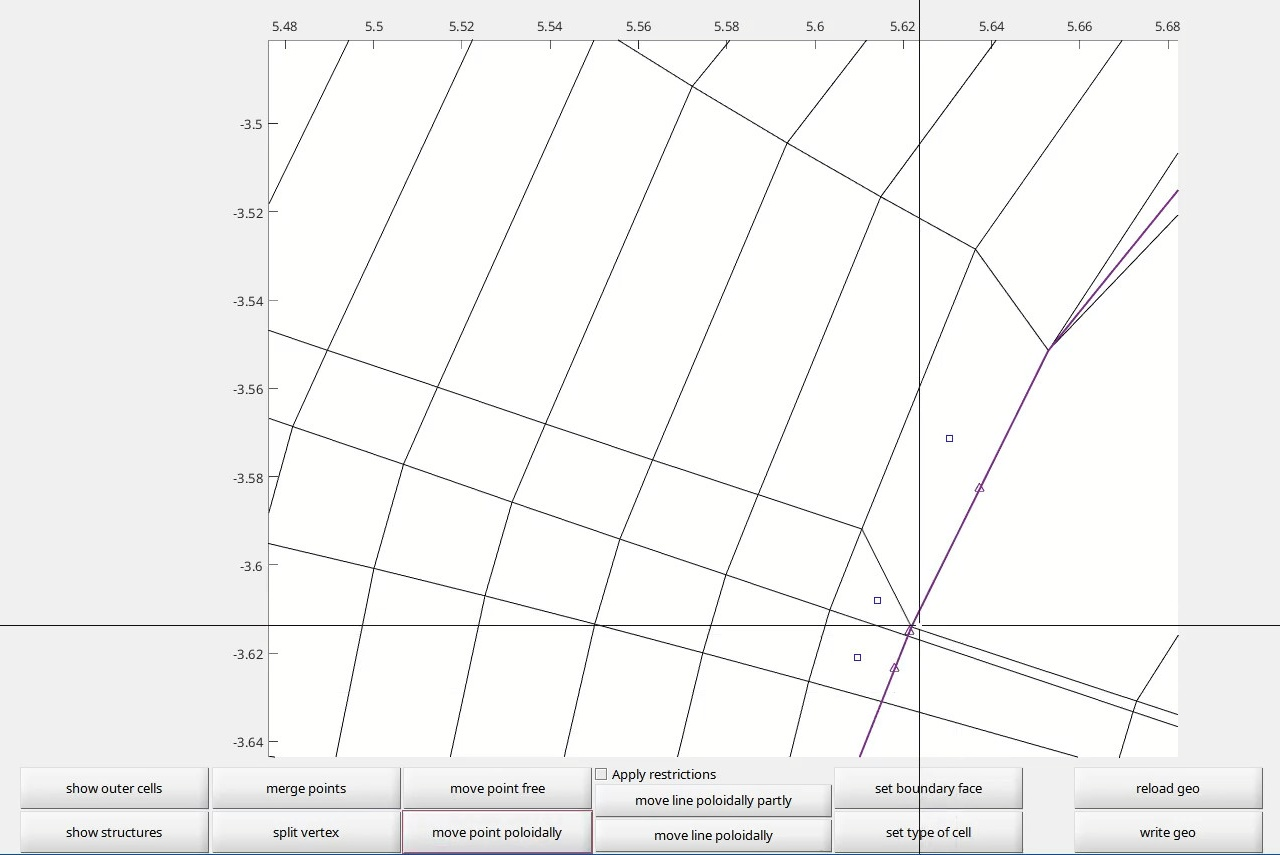
\includegraphics[width=0.333\linewidth]{pictures/move_point1}
    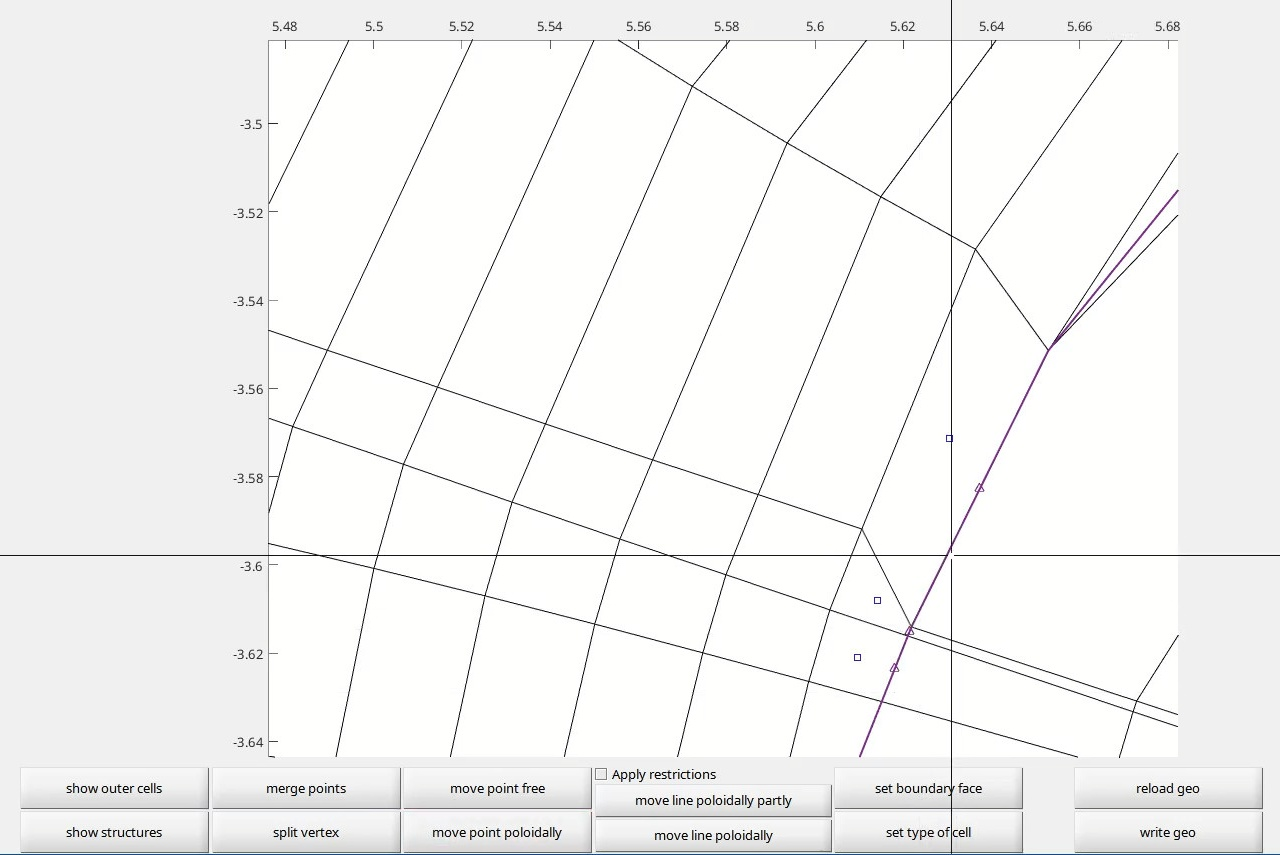
\includegraphics[width=0.333\linewidth]{pictures/move_point2}
    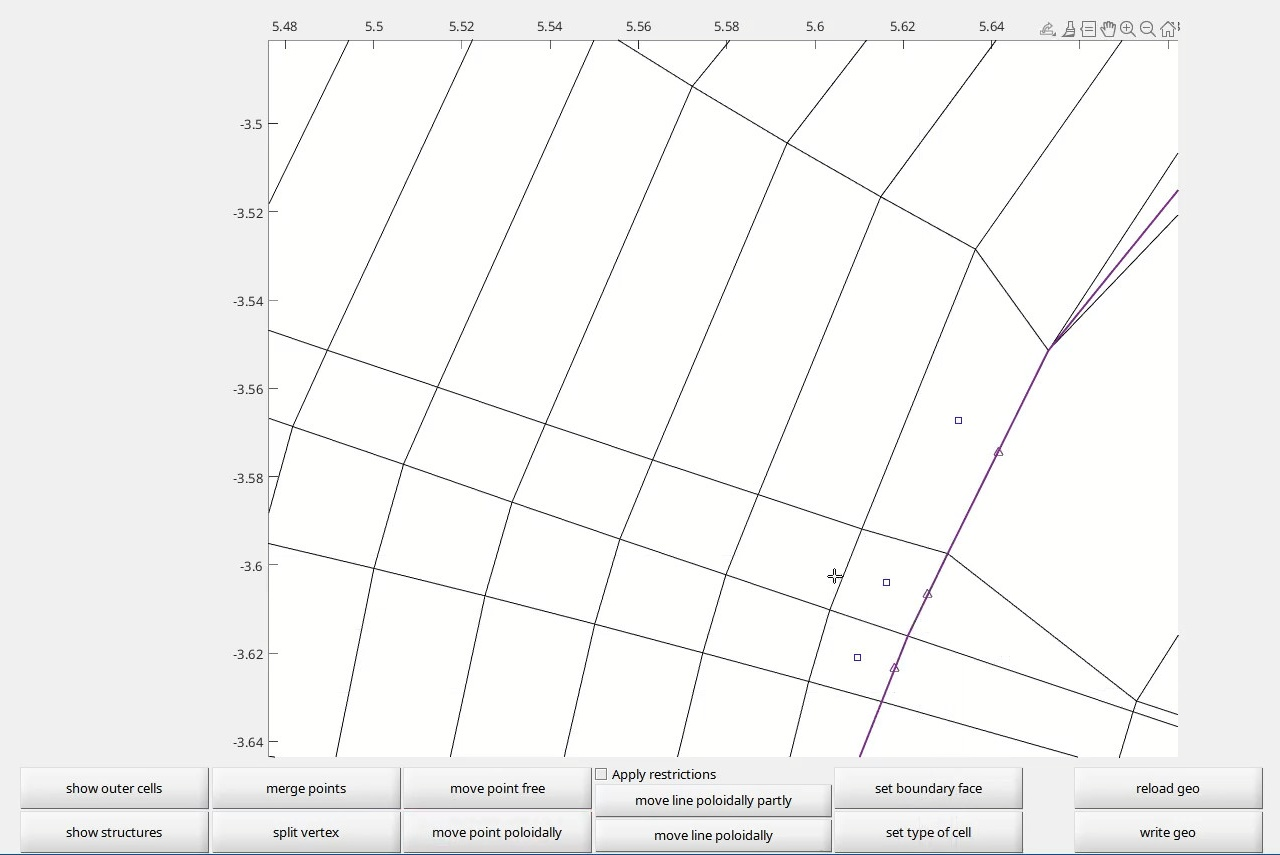
\includegraphics[width=0.333\linewidth]{pictures/move_point3}
    \caption{Adjusting boundary faces after line movement: (a) Select boundary vertex, (b) Move to target, (c) Result}
    \label{fig:movepoint_example}
  \end{figure}

  After moving this line, I repeated the same procedure for the region between the X-point and the inner divertor (see Figure~\ref{fig:moveline_example2}).

  \begin{figure}[H]
    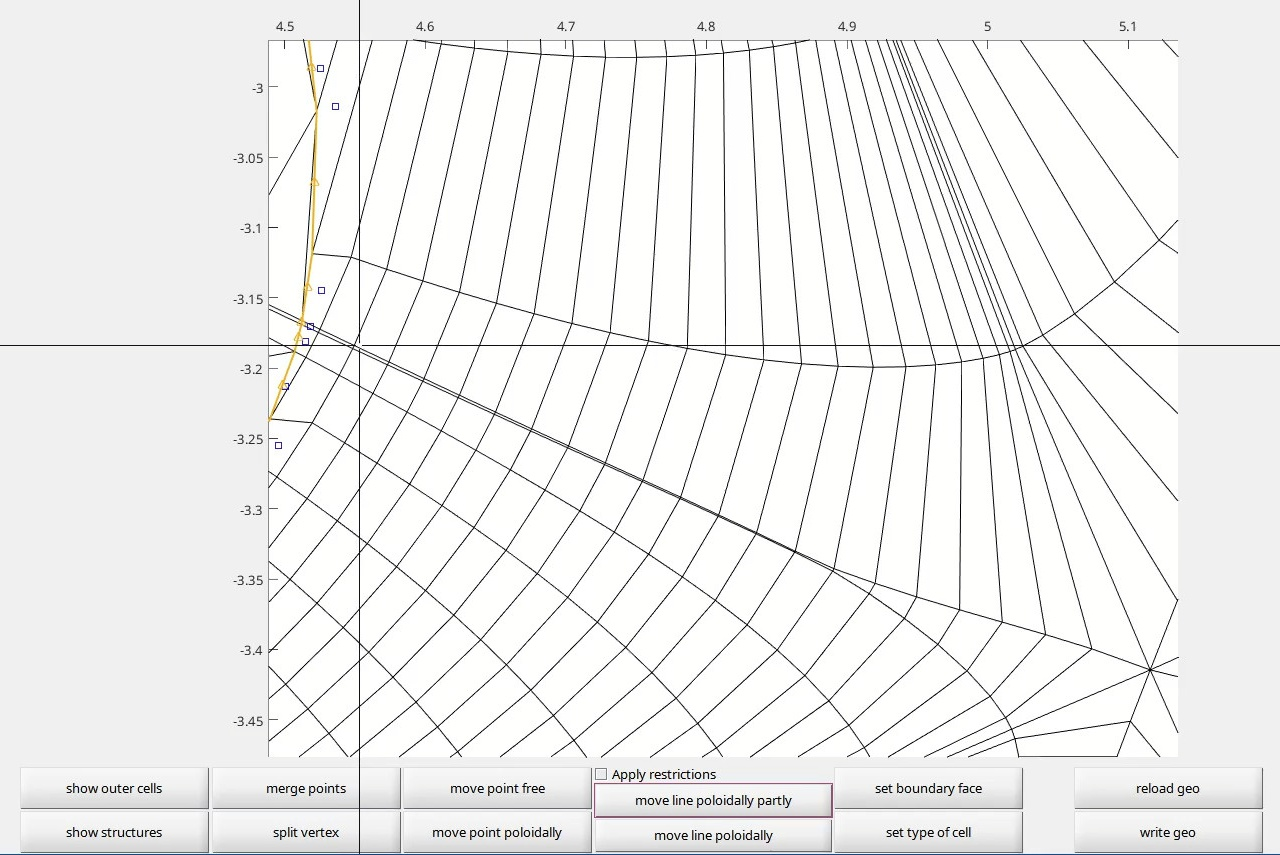
\includegraphics[width=0.5\linewidth]{pictures/move_line21}
    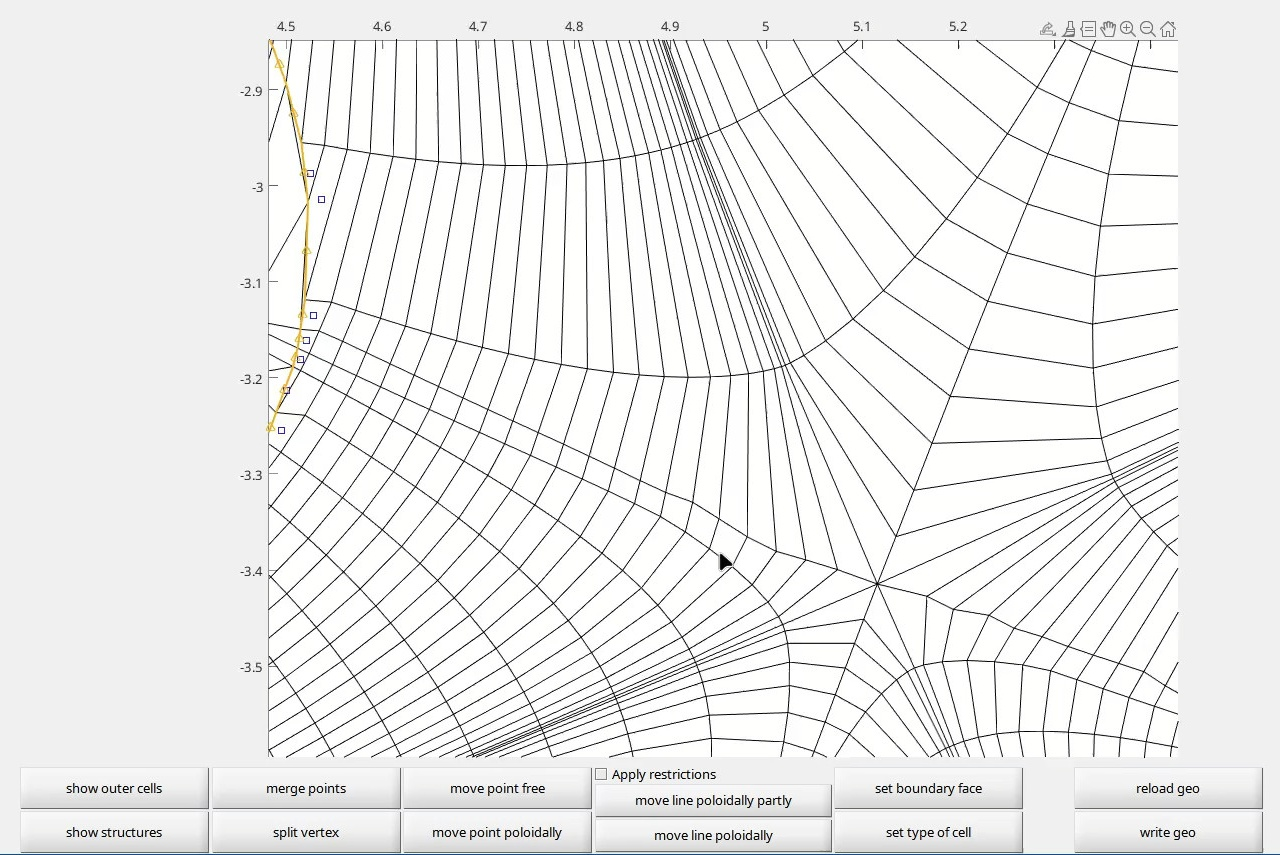
\includegraphics[width=0.5\linewidth]{pictures/move_line22}
    \caption{Movement of another line segment}
    \label{fig:moveline_example2}
  \end{figure}

  \subsection{Correcting Boundary Definition Errors}

  Next, I examined the boundary for definition errors. Figure~\ref{fig:wrongface} shows an incorrectly defined boundary face (marked with a red ellipse) and an accompanying wrong boundary cell (cursor point). I corrected this using the {\tt Set Type of Cell} option, changing the cell type to {\tt Inner}.

  \begin{figure}[H]
    \centering
    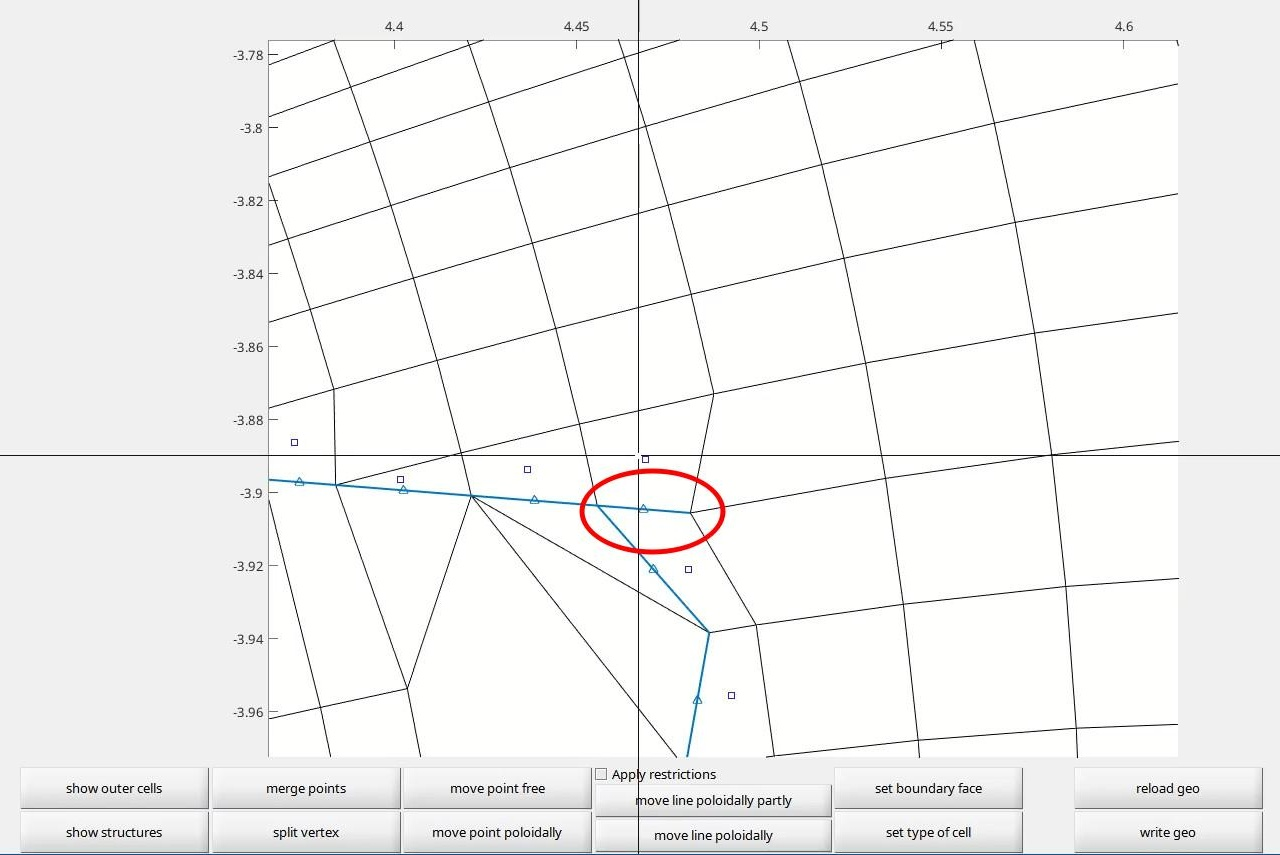
\includegraphics[width=0.5\linewidth]{pictures/wrong_face}
    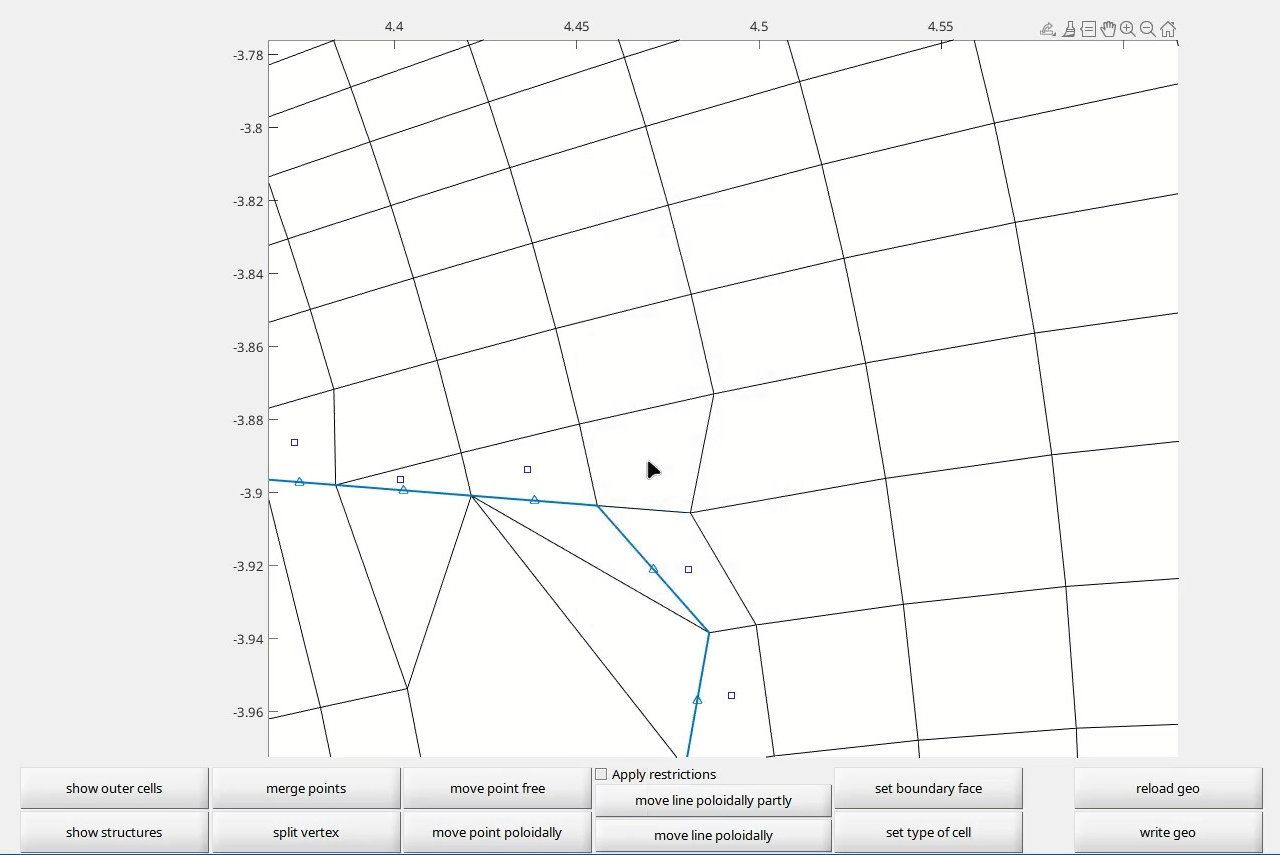
\includegraphics[width=0.5\linewidth]{pictures/wrong_face_corr}
    \caption{Incorrect boundary definition (left) and corrected configuration (right)}
    \label{fig:wrongface}
  \end{figure}

  \subsection{Reconstructing Mesh Structure}

  Figure~\ref{fig:correctcell1} presents a more complex example where I restructured face labels and connections to better align with the original geometry. This involved reassigning cell types and boundary definitions, as well as reconnecting a face using {\tt Split Vertex} and {\tt Merge Points} operations.

  \begin{figure}[H]
    \centering
    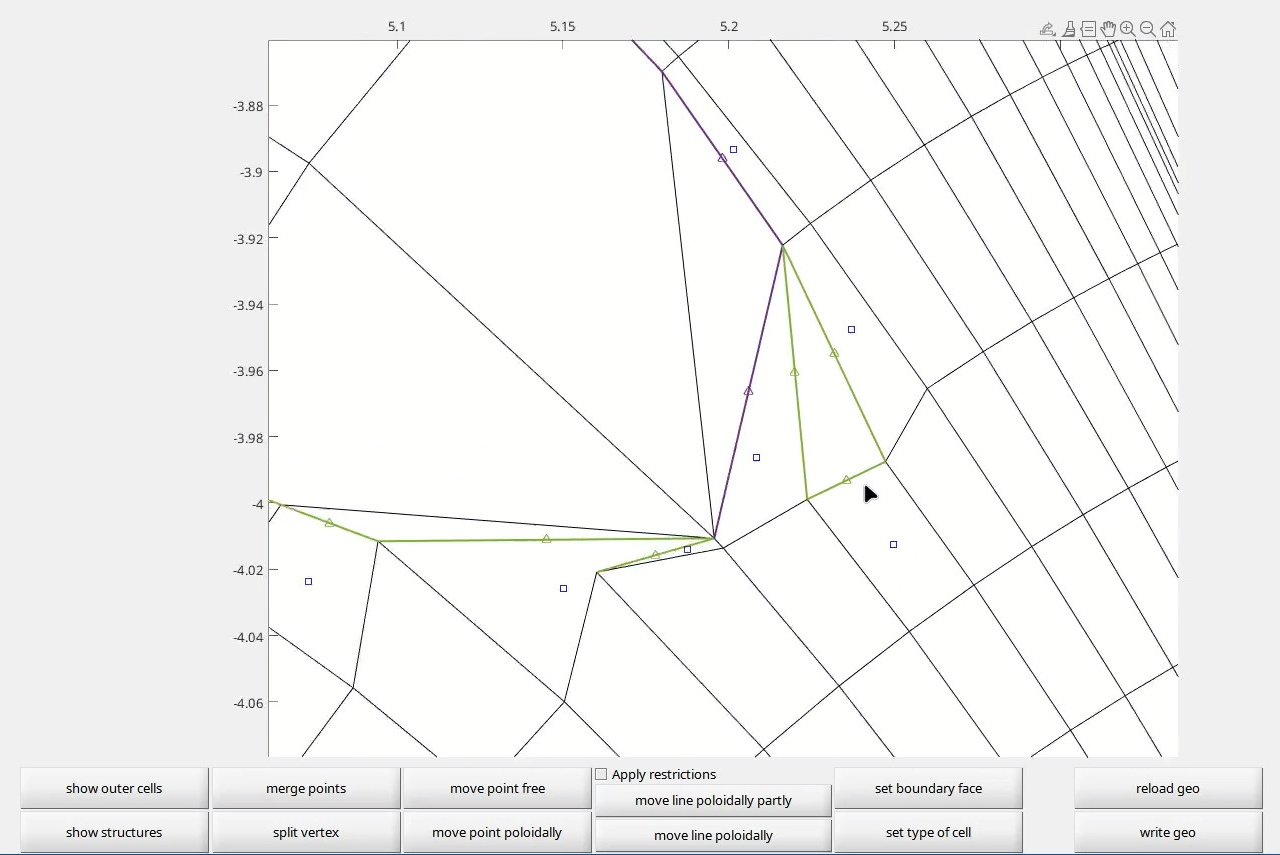
\includegraphics[width=0.5\linewidth]{pictures/correct_cell1}
    \caption{Area requiring structural modification}
    \label{fig:correctcell1}
  \end{figure}

  Figure~\ref{fig:splitvertex} illustrates the {\tt Split Vertex} operation. I selected the vertex to extract (left) and a new location for it (right). The exact position is not critical \textendash ~it can be placed anywhere convenient.

  \begin{figure}[H]
    \centering
    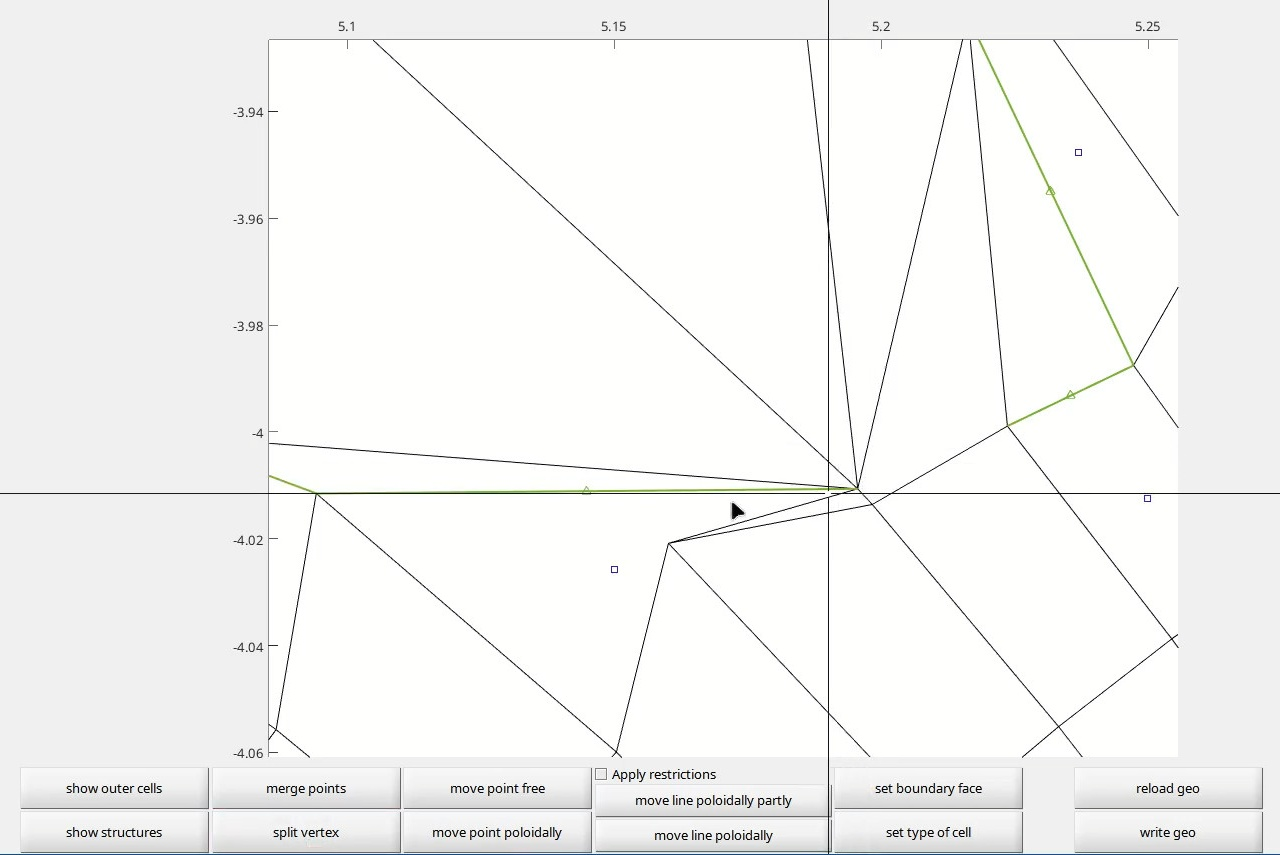
\includegraphics[width=0.5\linewidth]{pictures/split_vertex2}
    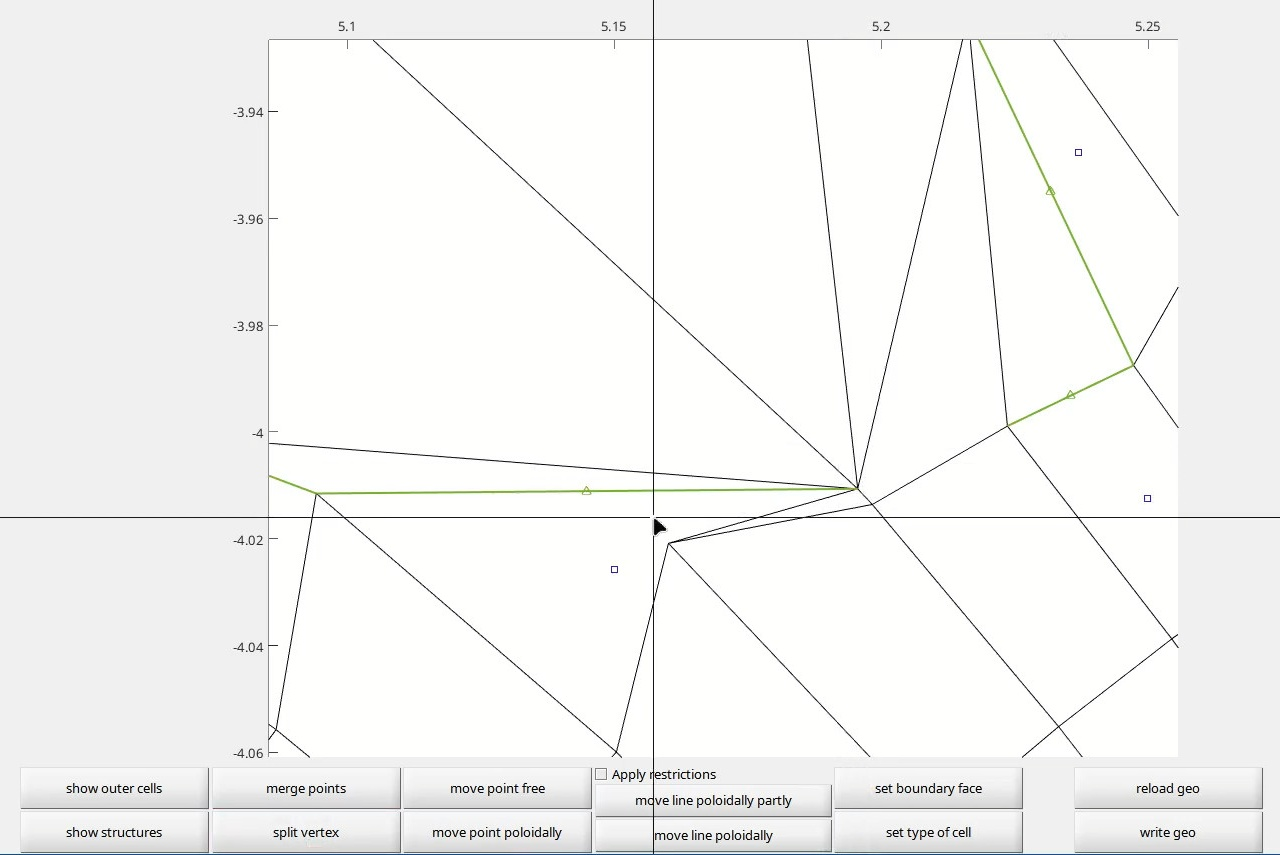
\includegraphics[width=0.5\linewidth]{pictures/split_vertex3}
    \caption{Splitting a vertex: selecting vertex to extract (left) and new location (right)}
    \label{fig:splitvertex}
  \end{figure}

  I then used {\tt Merge Points} (Figure~\ref{fig:mergepoints1}) to combine vertices: selecting the vertex to merge (left), choosing the target location (center), and observing the result (right).

  \begin{figure}[H]
    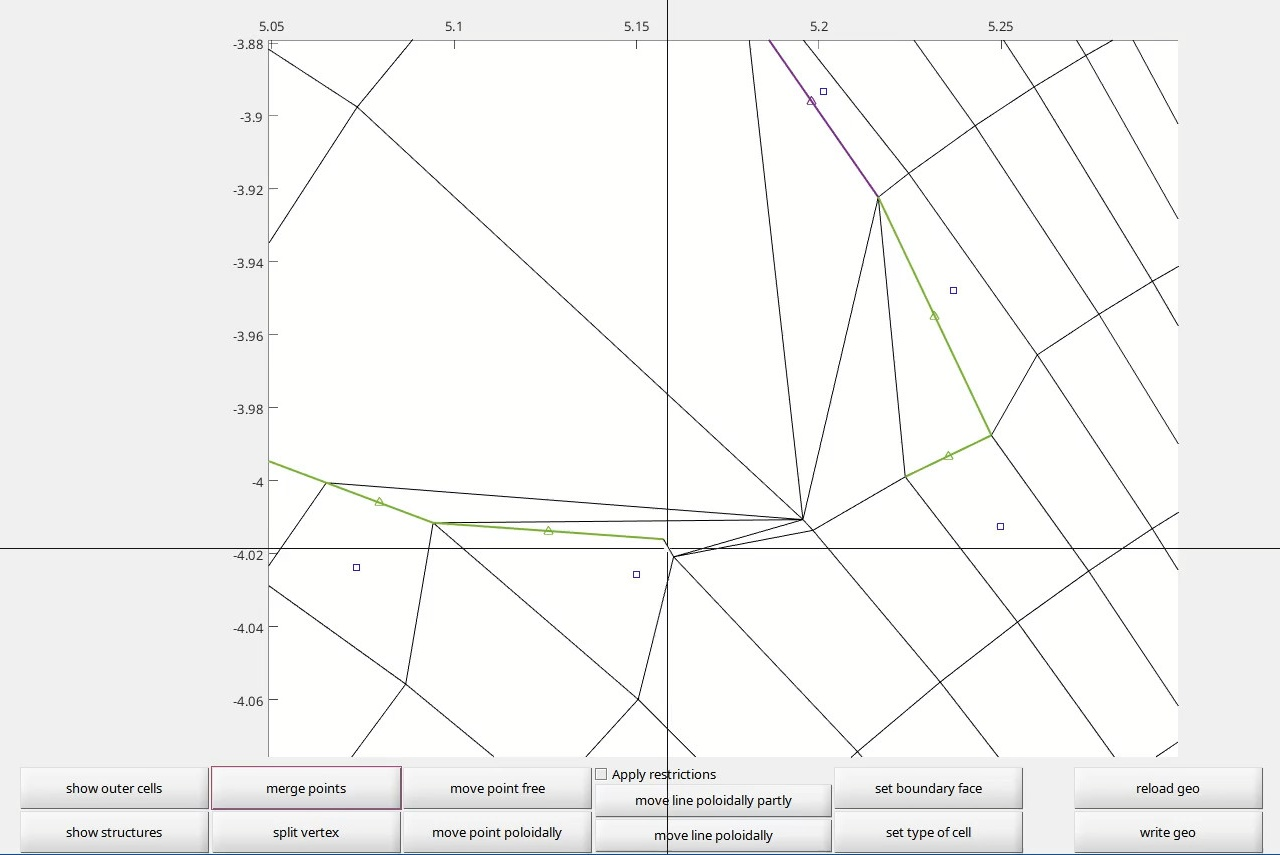
\includegraphics[width=0.333\linewidth]{pictures/merge_points1}
    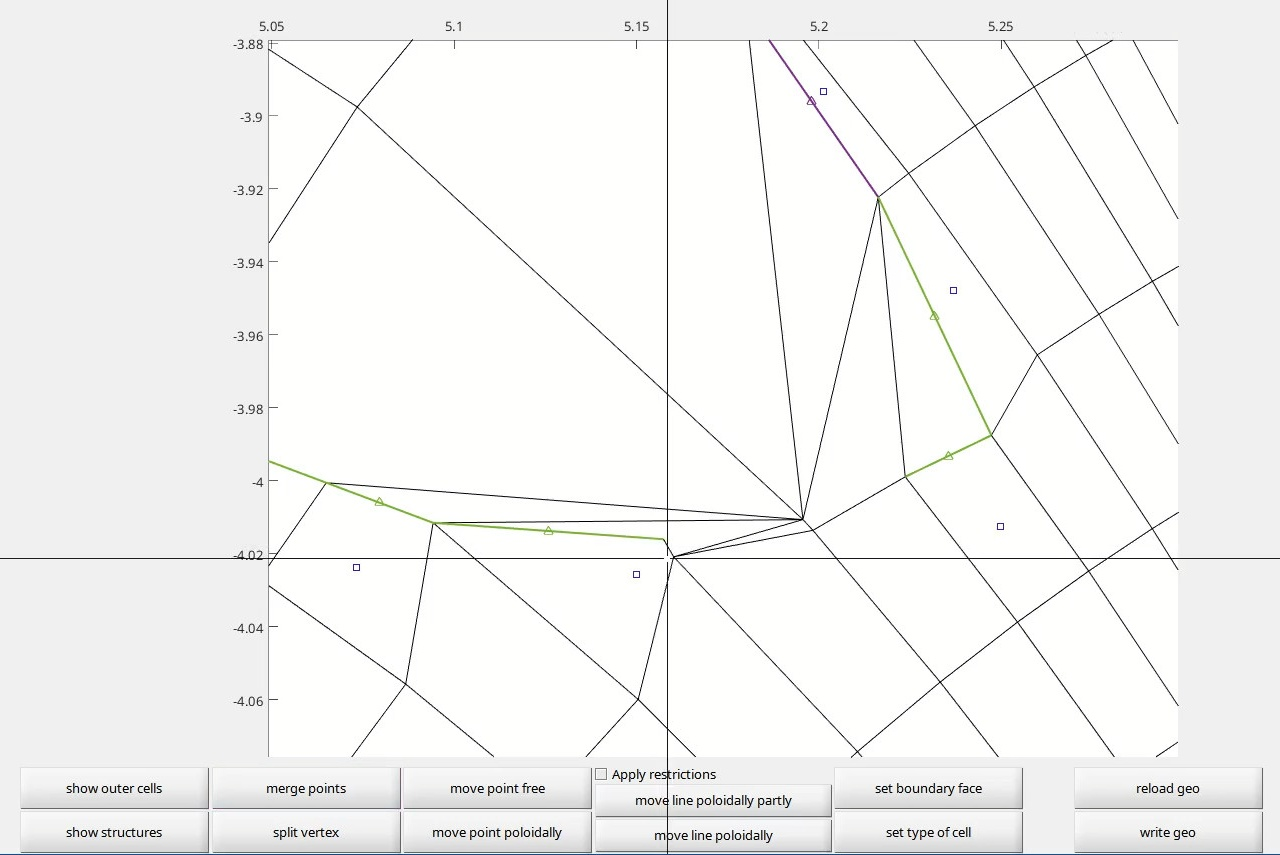
\includegraphics[width=0.333\linewidth]{pictures/merge_points2}
    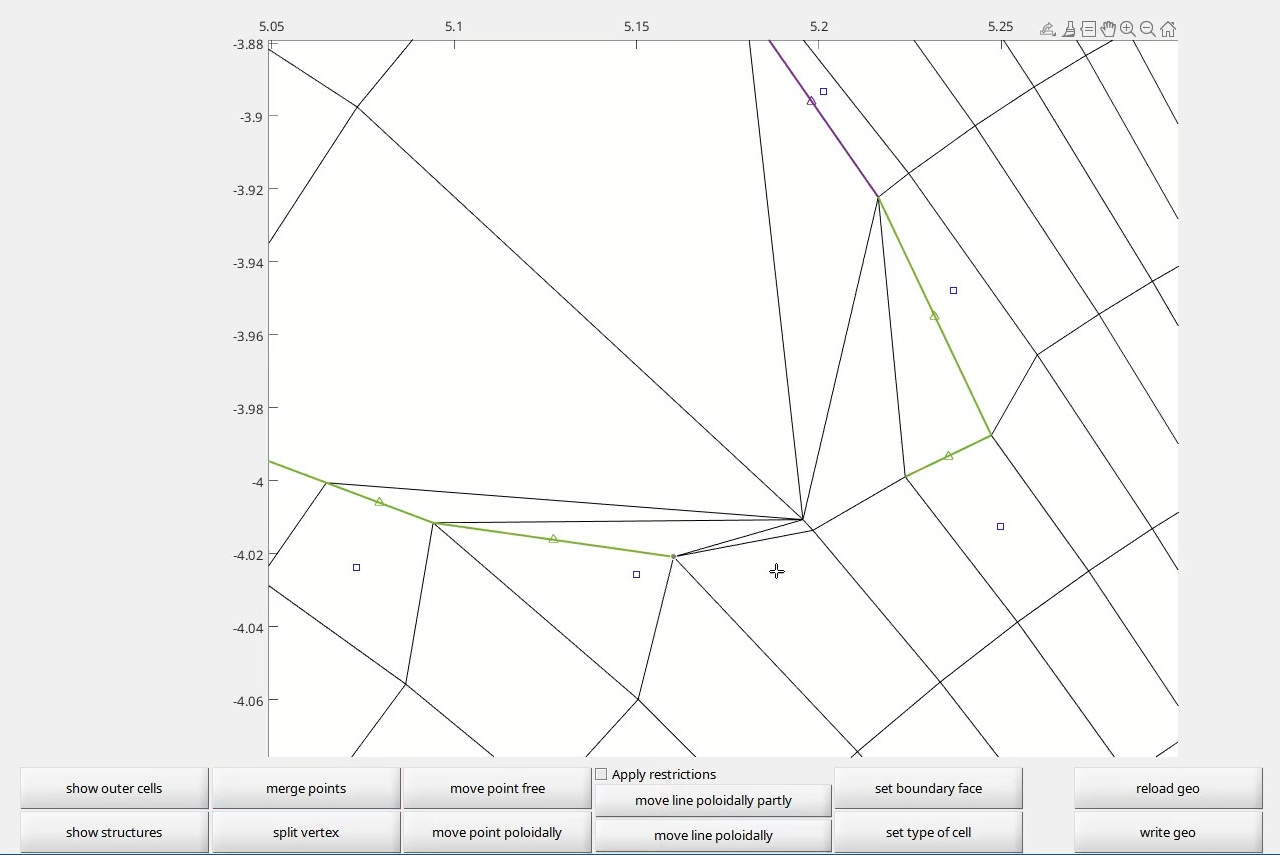
\includegraphics[width=0.333\linewidth]{pictures/merge_points3}
    \caption{Merging vertices: (a) Select vertex, (b) Select target, (c) Result}
    \label{fig:mergepoints1}
  \end{figure}

  Finally, I marked two faces as boundaries to close the polygon and saved this version as a backup.

  \subsection{Removing Problematic Cells}

  I identified a flux tube containing only two cells and removed them by:
  \begin{enumerate}[itemsep=2pt,topsep=5pt]
    \item Setting both cells to {\tt Outer} using {\tt Set Type of Cell}
    \item Marking two adjacent cells as boundaries using {\tt Set Boundary Face} to maintain polygon closure
  \end{enumerate}
  Figure~\ref{fig:remove_ft} shows the configuration before and after removal.

  \begin{figure}[H]
    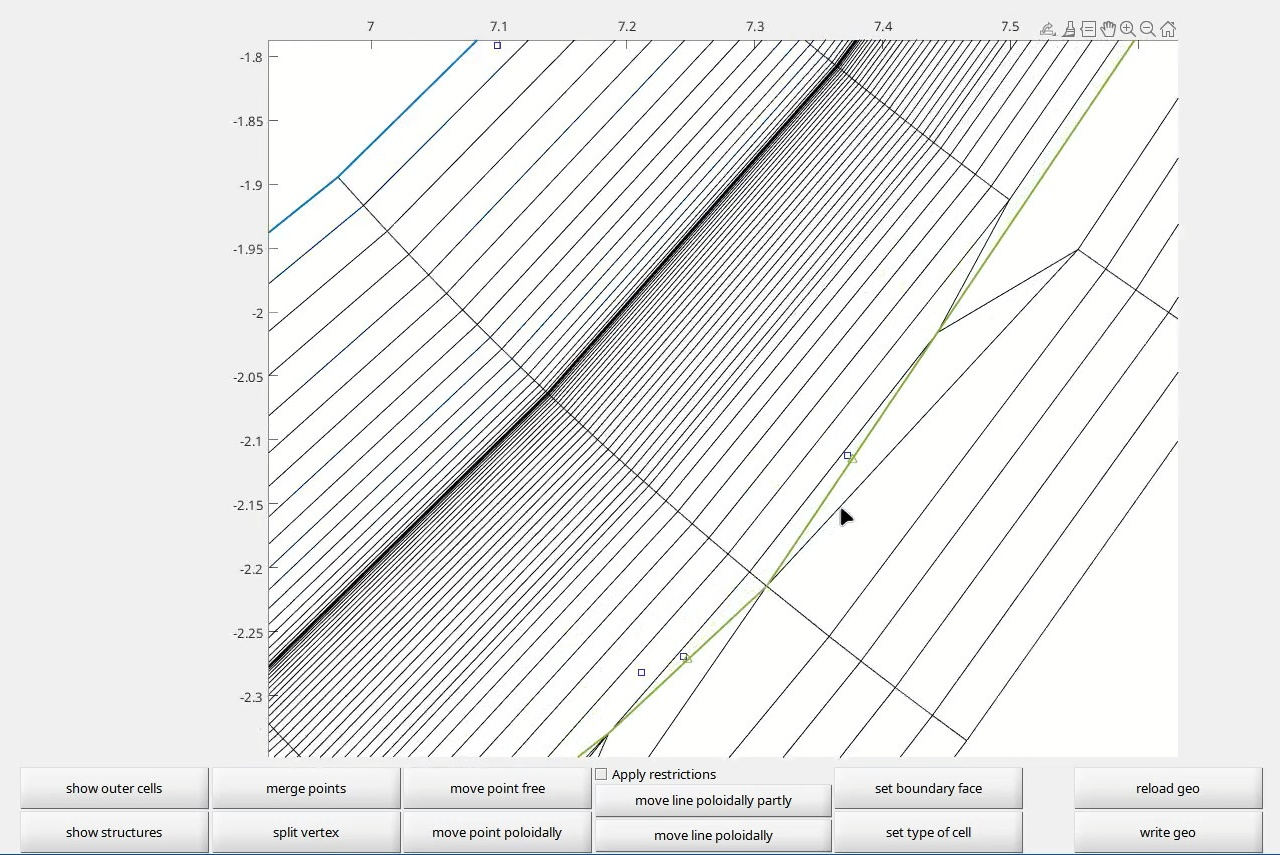
\includegraphics[width=0.5\linewidth]{pictures/remove_ft1}
    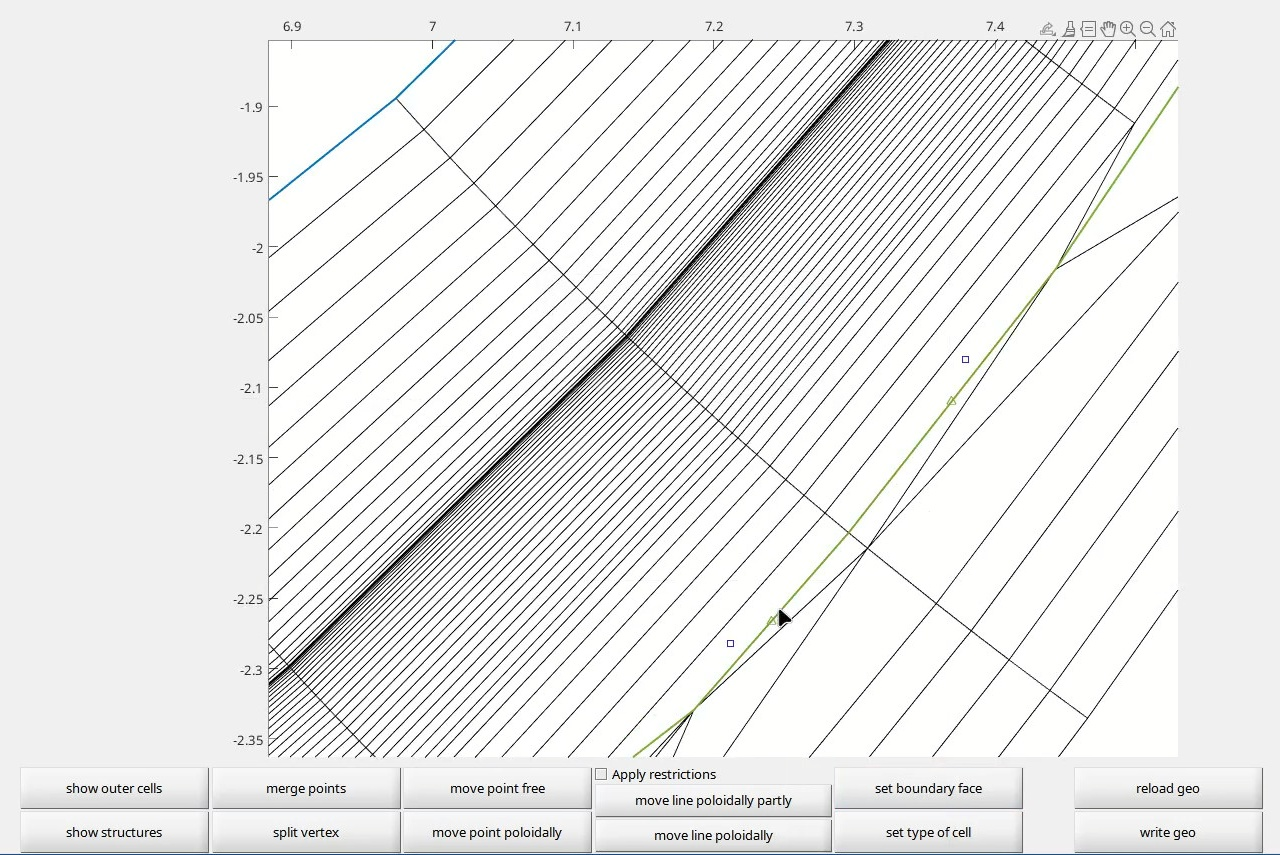
\includegraphics[width=0.5\linewidth]{pictures/remove_ft2}
    \caption{Removing a short flux tube: before (left) and after (right)}
    \label{fig:remove_ft}
  \end{figure}

  Another problematic area contained a very small cell that could cause numerical issues. I eliminated it through the following steps (Figure~\ref{fig:smallcell}):
  \begin{enumerate}[itemsep=2pt,topsep=5pt]
    \item Set the small cell type to {\tt Outer}
    \item Set the neighbouring cell to {\tt Boundary} and defined its corresponding face as a boundary
    \item Merged the red vertex into the blue vertex (using {\tt Merge Points})
  \end{enumerate}

  \begin{figure}[H]
    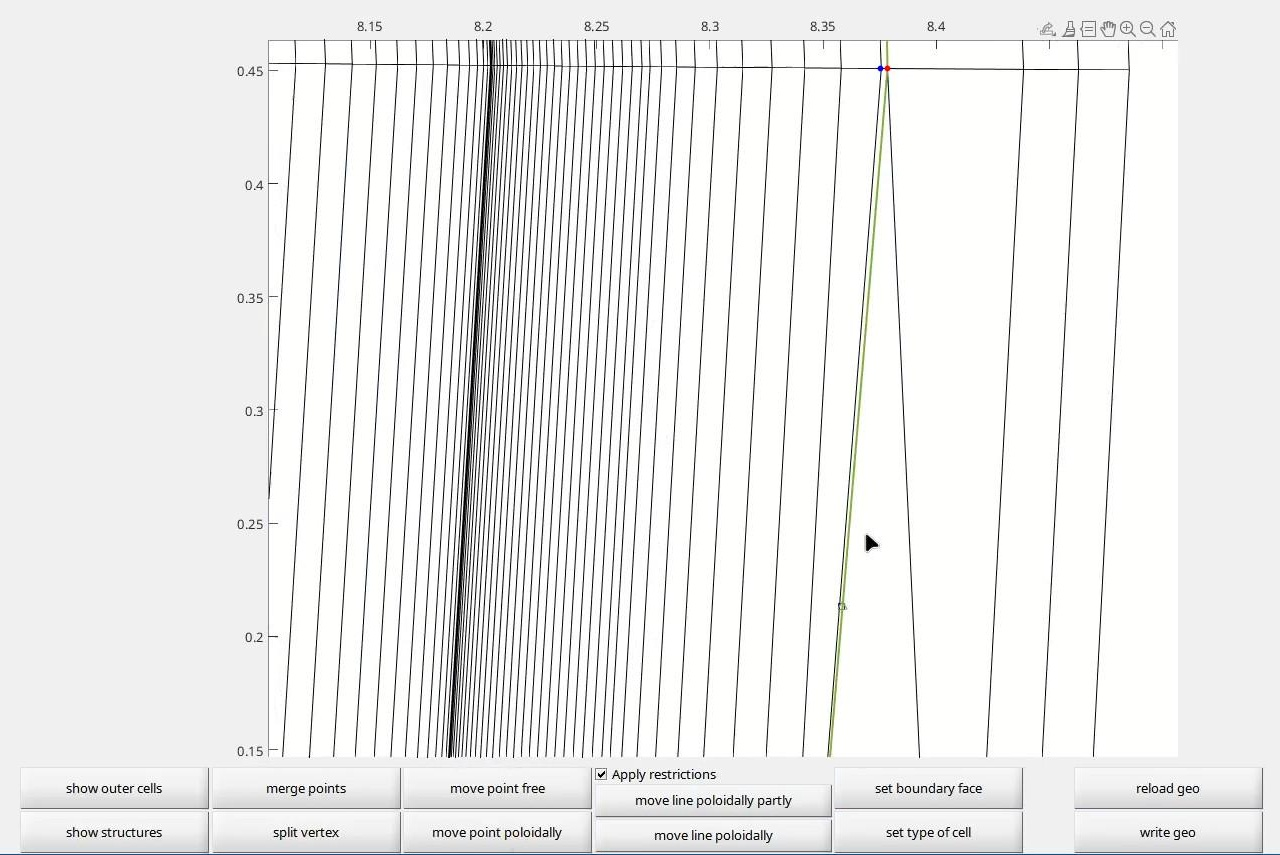
\includegraphics[width=0.5\linewidth]{pictures/small_cell1_edit}
    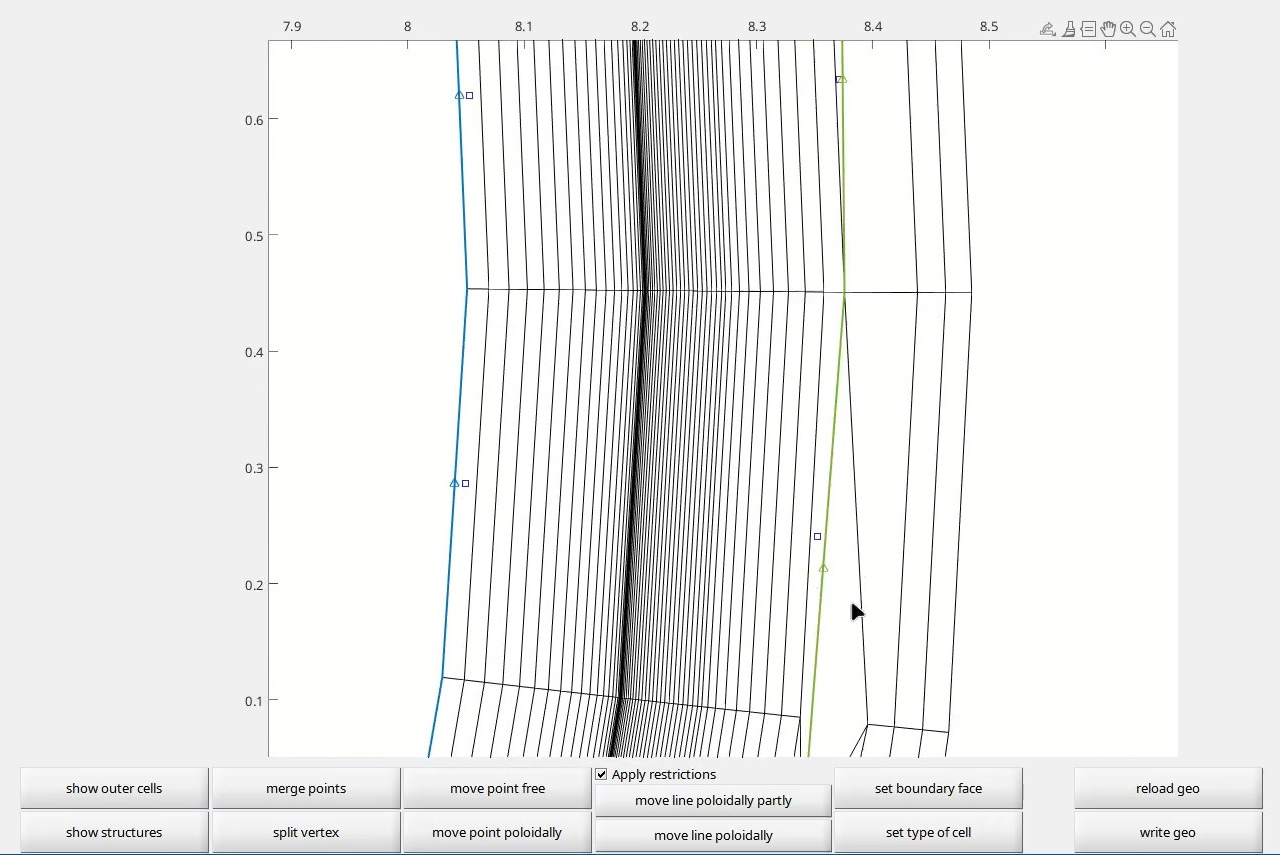
\includegraphics[width=0.5\linewidth]{pictures/small_cell2}
    \caption{Eliminating a small cell: before (left) and after (right)}
    \label{fig:smallcell}
  \end{figure}

  \subsection{Correcting Distorted Faces}

  I then corrected an unnecessarily distorted face using {\tt Move Point Free}, as shown in Figure~\ref{fig:movepointfree}.

  \begin{figure}[H]
    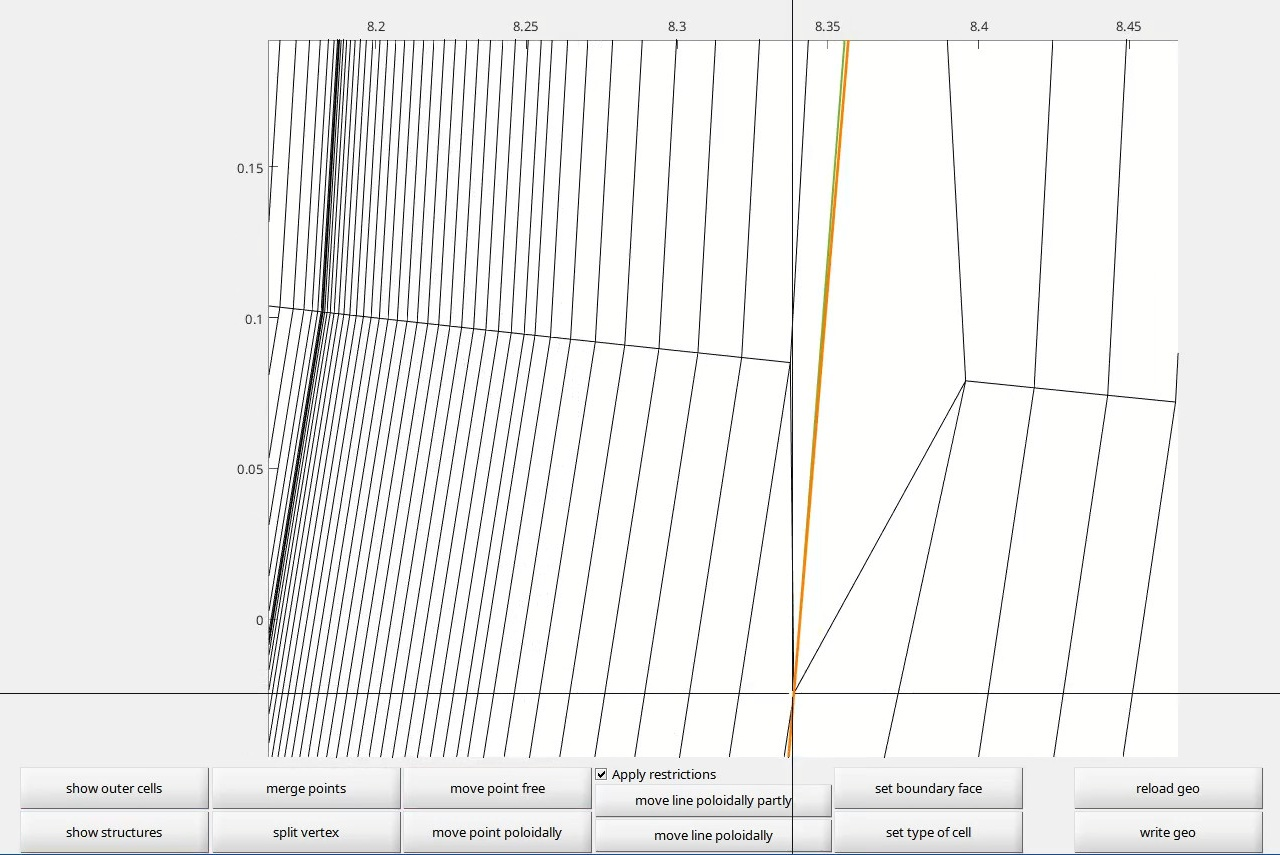
\includegraphics[width=0.333\linewidth]{pictures/move_point_free1}
    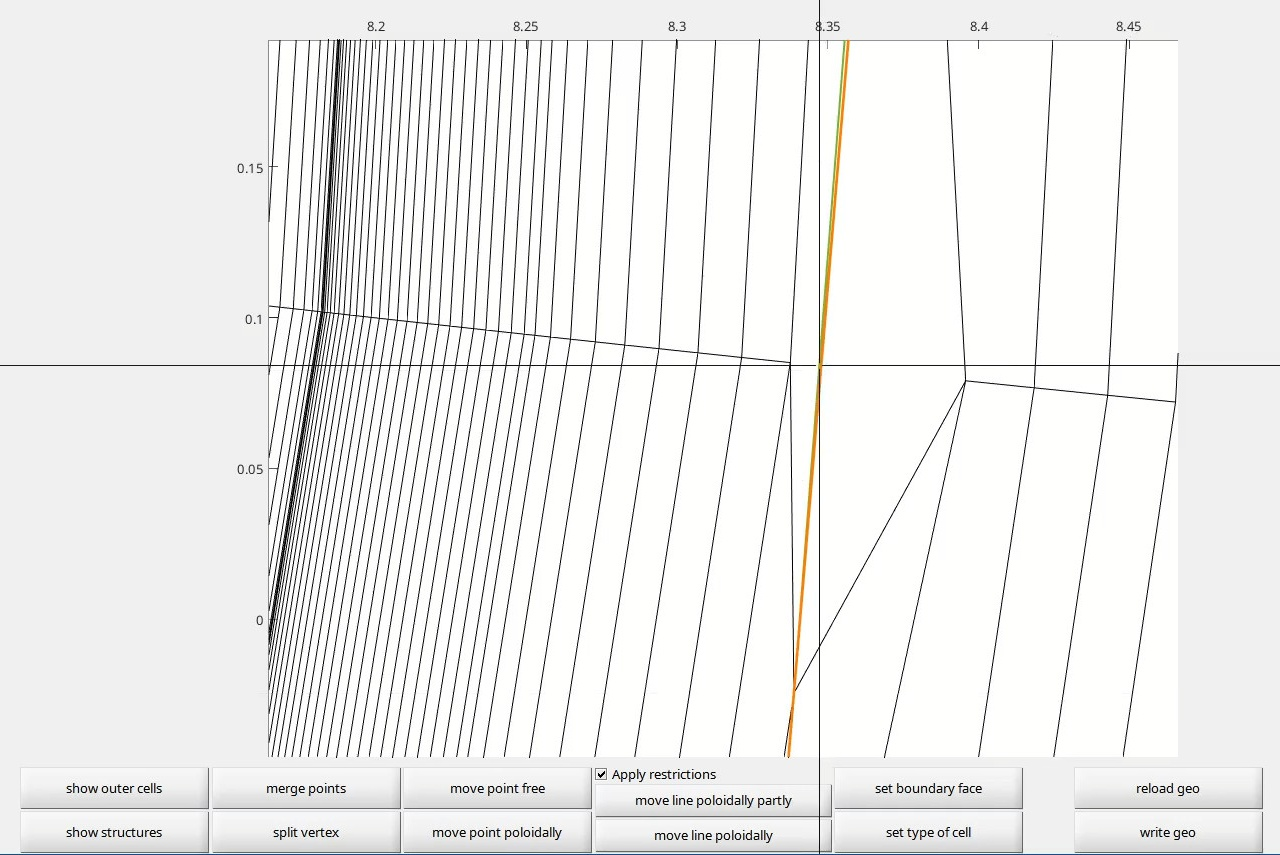
\includegraphics[width=0.333\linewidth]{pictures/move_point_free2}
    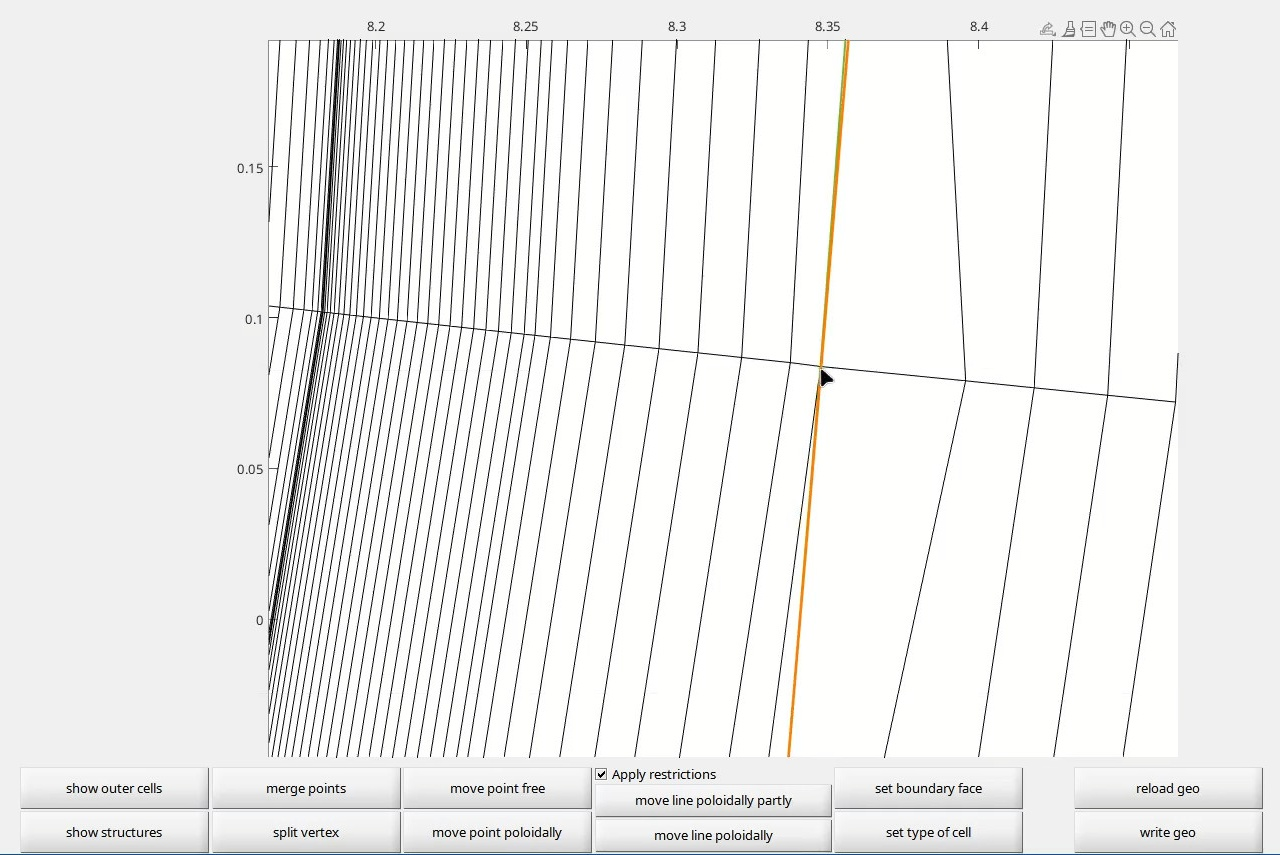
\includegraphics[width=0.333\linewidth]{pictures/move_point_free3}
    \caption{Correcting a distorted face using free point movement}
    \label{fig:movepointfree}
  \end{figure}

  \subsection{Removing a Narrow Flux Tube}

  Finally, I removed a narrow flux tube along the wall and reconstructed the wall using an adjacent flux tube. This involved four steps:
  \begin{enumerate}[itemsep=2pt,topsep=5pt]
    \item Marked all cells in the narrow flux tube as {\tt Outer} using {\tt Set Type of Cell}
    \item Merged vertices of the neighboring flux tube into the wall vertices using {\tt Merge Vertex}
    \item Marked faces of the neighboring flux tube as boundary faces using {\tt Set Boundary Face}
  \end{enumerate}

  \begin{figure}[H]
    \centering
    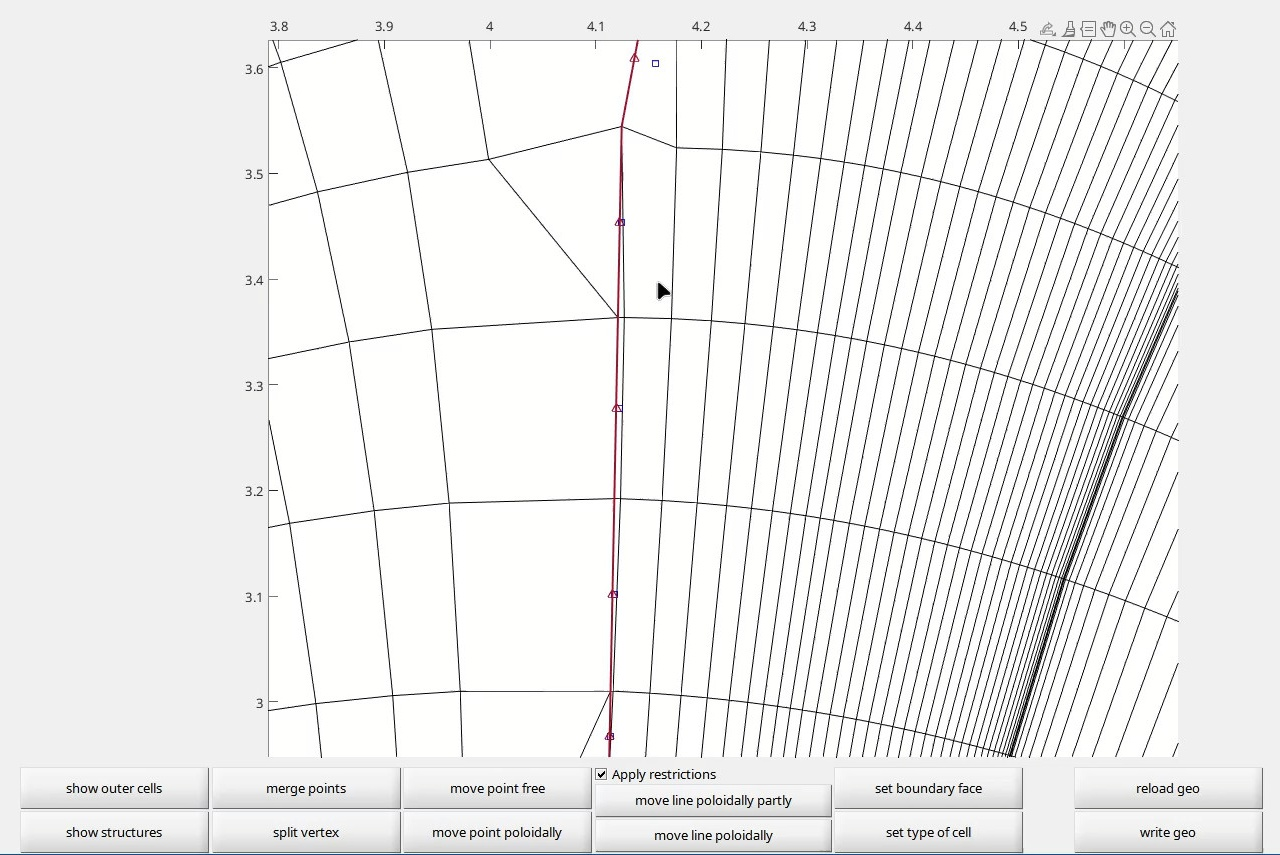
\includegraphics[width=0.245\linewidth]{pictures/remove_ft21}
    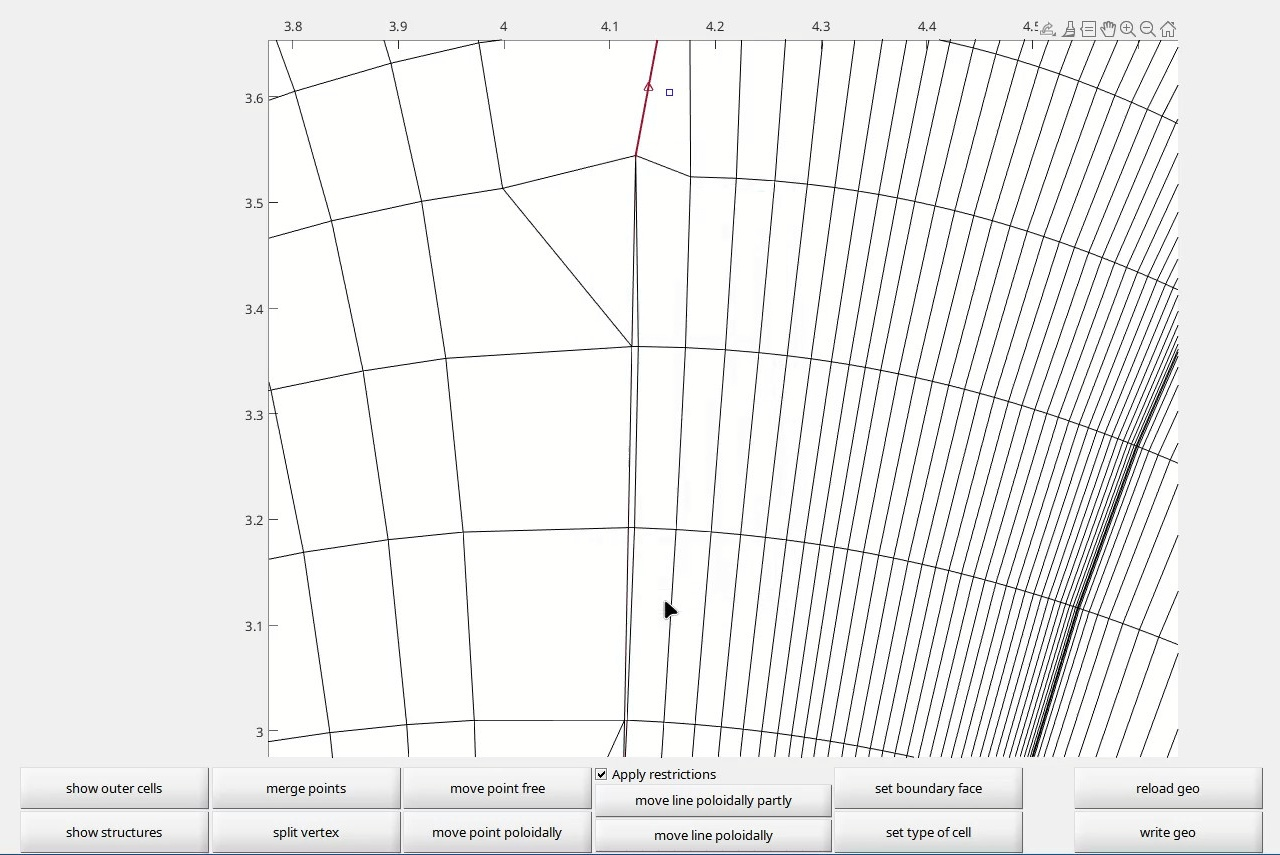
\includegraphics[width=0.245\linewidth]{pictures/remove_ft22}
    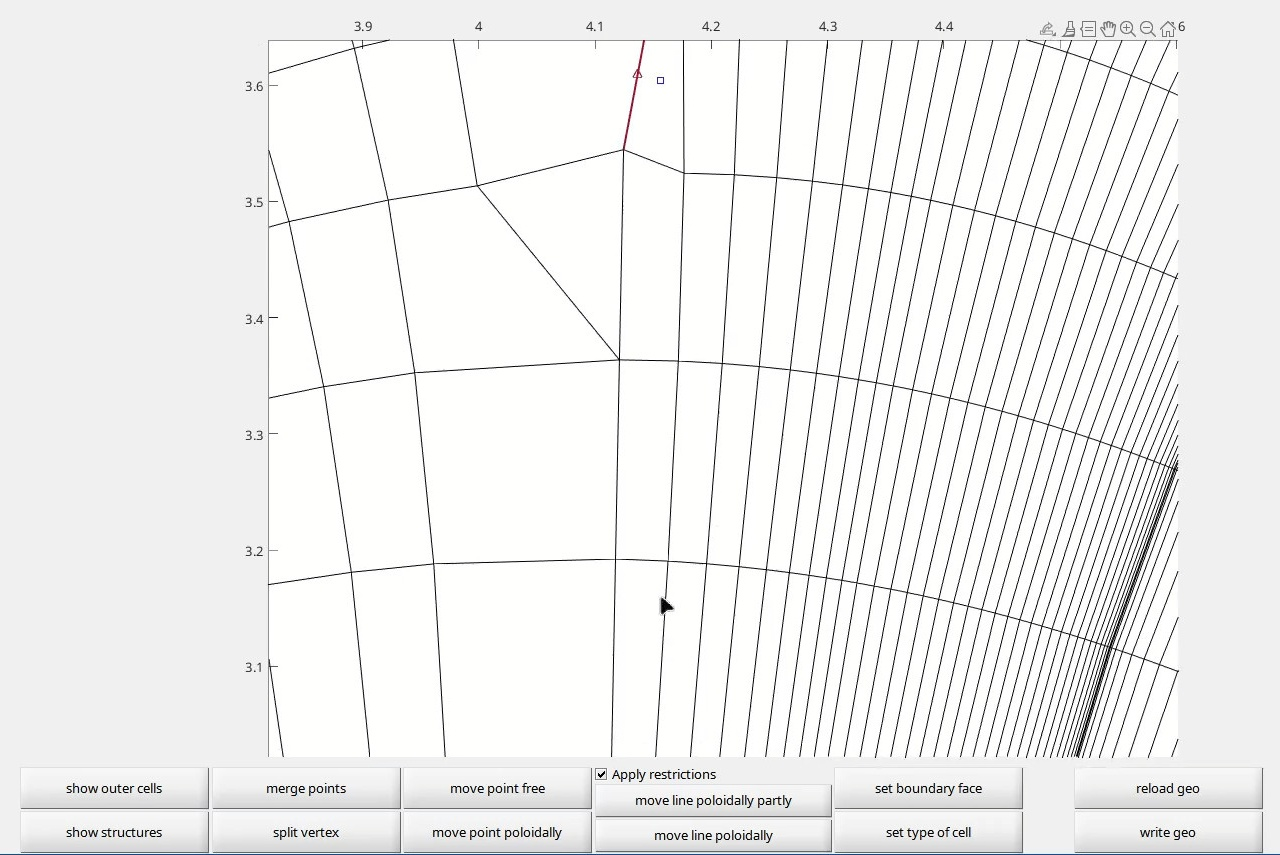
\includegraphics[width=0.245\linewidth]{pictures/remove_ft23}
    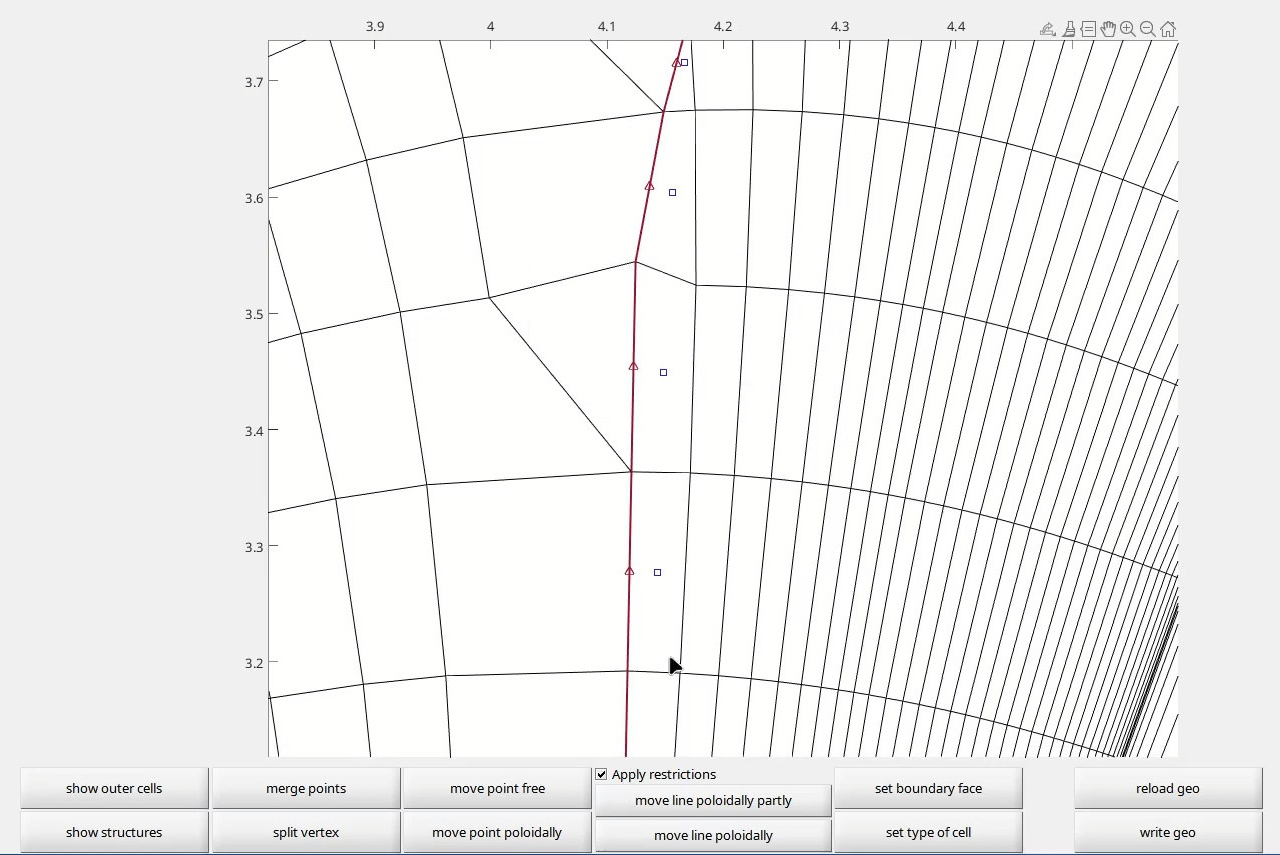
\includegraphics[width=0.245\linewidth]{pictures/remove_ft24}
    \caption{Removing a narrow flux tube: (a) Initial state, (b) Cells marked as outer, (c) Vertices merged, (d) Boundary faces defined}
    \label{fig:remove_flux_tube_sequence}
  \end{figure}

  Other mesh modifications performed were similar to the examples described above.
\end{document}
